% This must be in the first 5 lines to tell arXiv to use pdfLaTeX, which is strongly recommended.
\pdfoutput=1
% In particular, the hyperref package requires pdfLaTeX in order to break URLs across lines.

\documentclass[11pt]{article}

% Change "review" to "final" to generate the final (sometimes called camera-ready) version.
% Change to "preprint" to generate a non-anonymous version with page numbers.
\usepackage[final]{acl}

% Standard package includes
\usepackage{times}
\usepackage{latexsym}
% \usepackage[pagebackref,breaklinks,colorlinks,citecolor=cvprblue]{hyperref}
\usepackage{multirow}
\usepackage{booktabs}
% For proper rendering and hyphenation of words containing Latin characters (including in bib files)
\usepackage[T1]{fontenc}
% For Vietnamese characters
% \usepackage[T5]{fontenc}
% See https://www.latex-project.org/help/documentation/encguide.pdf for other character sets

% This assumes your files are encoded as UTF8
\usepackage[utf8]{inputenc}

\usepackage{microtype}
\usepackage{graphicx}
\usepackage{subcaption}
\usepackage{amsmath}
\usepackage{cleveref}
\usepackage{tcolorbox}

\usepackage{amssymb}
\usepackage{xcolor}
\usepackage{pifont}
\definecolor{my_green}{RGB}{51,102,0}
\definecolor{my_red}{RGB}{204, 0, 0}
\newcommand{\cmark}{\textcolor{my_green}{\ding{51}}} % ✔
\newcommand{\xmark}{\textcolor{my_red}{\ding{55}}} % ✘
\newcommand{\lilei}[1]{\textcolor{violet}{\bf \small [#1 --lilei]}}
\newcommand{\lpk}[1]{\textcolor{blue}{\bf \small [#1 --lpk]}}

% This is also not strictly necessary, and may be commented out.
% However, it will improve the aesthetics of text in
% the typewriter font.
\usepackage{inconsolata}

% If the title and author information does not fit in the area allocated, uncomment the following
%
%\setlength\titlebox{<dim>}
%
% and set <dim> to something 5cm or larger.

\title{Multimodal ArXiv: A Dataset for Improving Scientific Comprehension of Large Vision-Language Models}

% Author information can be set in various styles:
% For several authors from the same institution:
% \author{Author 1 \and ... \and Author n \\
%         Address line \\ ... \\ Address line}
% if the names do not fit well on one line use
%         Author 1 \\ {\bf Author 2} \\ ... \\ {\bf Author n} \\
% For authors from different institutions:
% \author{Author 1 \\ Address line \\  ... \\ Address line
%         \And  ... \And
%         Author n \\ Address line \\ ... \\ Address line}
% To start a separate ``row'' of authors use \AND, as in
% \author{Author 1 \\ Address line \\  ... \\ Address line
%         \AND
%         Author 2 \\ Address line \\ ... \\ Address line \And
%         Author 3 \\ Address line \\ ... \\ Address line}

\author{
Lei Li\thanks{Equal Contribution.}$^\dagger$,  Yuqi Wang$^*$$^\dagger$, Runxin Xu$^\ddag$, Peiyi Wang$^\ddag$\\\textbf{Xiachong Feng$^\dagger$, Lingpeng Kong$^\dagger$, Qi Liu$^\dagger$}\\ 
$^\dagger$The University of Hong Kong \\
$^\ddagger$Peking University\\
 \texttt{\{nlp.lilei, runxinxu, wangpeiyi9979, xiachongfeng1996\}@gmail.com} \\ 
 \texttt{wangyuqi@connect.hku.hk} \quad \texttt{\{lpk, liuqi\}@cs.hku.hk}\\
  }
\def\DatasetName{ArXivCap\ }

\begin{document}
\maketitle
\enlargethispage{2\baselineskip}
\begin{abstract}
Foundation model development attracts a rapidly expanding body of contributors, scientists, and applications.
To help shape \emph{responsible development practices}, we introduce the Foundation Model Development Cheatsheet: a growing collection of 250+ tools and resources spanning text, vision, and speech modalities.
We draw on a large body of prior work to survey resources (\emph{e.g.} software, documentation, frameworks, guides, and practical tools) that support informed data selection, processing, and understanding, precise and limitation-aware artifact documentation, efficient model training, advance awareness of the environmental impact from training, careful model evaluation of capabilities, risks, and claims, as well as responsible model release, licensing and deployment practices.
We hope this curated collection of resources helps guide more responsible development.
The process of curating this list, enabled us to review the AI development ecosystem, revealing what tools are critically missing, misused, or over-used in existing practices.
We find that (i) tools for data sourcing, model evaluation, and monitoring are critically under-serving ethical and real-world needs, (ii) evaluations for model safety, capabilities, and environmental impact all lack reproducibility and transparency, (iii) text and particularly English-centric analyses continue to dominate over multilingual and multi-modal analyses, and (iv) evaluation of systems, rather than just models, is needed so that capabilities and impact are assessed in context.  %\TODO{Finish one more point on systems vs models?}
% We hope this survey and review of resources will provide a practical guide to developers and a compass for meaningful future work in responsible AI.
\end{abstract}
% (\href{http://fmcheatsheet.org}{fmcheatsheet.org})



\section{Introduction}
\label{sec:intro}

% The evolution of Large Language Models (LLMs)~\citep{gpt3,touvron2023llama,chatgpt} and vision foundation models~\citep{radford2021clip}
% has catalyzed advancements in constructing multi-modal intelligent agents capable of exploring the multi-modal realm, which are achieved by integrating LLMs and pre-trained vision encoders, followed by fine-tuning on image-text pairs~\citep{madureira-2021-flamingos,awadalla2023openflamingo} or specifically curated vision instruction-tuning datasets~\citep{liu2023llava,li2023m3it,Qwen-VL}.
% The evolution of Large Language Models (LLMs)~\citep{gpt3,touvron2023llama,chatgpt} and vision foundation models~\citep{radford2021clip} has catalyzed advancements in constructing intelligent agents capable of processing multi-modal information. 
Large vision-language models (LVLMs), which integrate large language models (LLMs)~\citep{gpt3,touvron2023llama} with pre-trained vision encoders through cross-modal alignment training~\citep{madureira-2021-flamingos,liu2023llava,li2023m3it}, 
have demonstrated remarkable perceptual and cognitive capabilities in processing concrete images from everyday scenes~\citep{gpt4v,fu2023mme,yang2023dawn,reka2024core}.
However, recent studies have shown that open-source LVLMs struggle to understand abstract figures, such as geometric shapes in multimodal mathematical reasoning~\citep{mathvista,zhang2024mathverse} and scientific plots~\citep{mmmu}. 
The inadequacy of training datasets in scientific domains that involve complex reasoning with abstract figures is the main underlying cause.
% This limitation stems from the scarcity of training datasets in scientific domains that incorporate complex reasoning involving abstract figures.
% , as most multi-modal instruction datasets focus on general images
% However, it remains unclear \lpk{if we know it's basically not satisfactory, then we can say it's not good rather than remains unclear} whether LVLMs can effectively reason over scientific figures and generate concise, human-like summary descriptions for paper figures. 
% This inquiry holds significance on two fronts: from a scientific perspective, it offers an ideal testbed for examining whether LVLMs can handle complex semantics involving reasoning processes that go beyond what is required by traditional vision question-answering~(QA) tasks. On a practical level, the implementation of a machine-assisted captioning tool could significantly enhance research efficiency, rendering scientific figures more accessible for individuals with visual impairments. \lpk{left here.}
% traditional vision-language tasks have 

To address this, we construct Multimodal ArXiv by utilizing the rich resources in preprints hosted on arXiv to improve the ability to understand scientific literature in LVLMs.
We first curate ArXivCap, a
diverse scientific figure-caption dataset.
In contrast to previous scientific figure datasets, which consist of synthesized figures~\citep{chen2020figcap}
or are restricted to simple captioning scenarios in the computer science domain~\citep{hsu-etal-2021-scicap-generating}, our dataset is composed of figures extracted from academic papers across a range of domains.
ArXivCap has 6.4M images and 3.9M captions from 572K papers. 
We also keep the subfigure structure, and titles of original papers, thereby supporting diverse evaluation tasks.
We further instruct GPT-4V to generate 100K multiple-choice question-answering~(QA) pairs for the figures in ArXivCap.
The resulting ArXivQA dataset could naturally serve as a pivotal resource for improving the scientific reasoning abilities of LVLMs.

We validate the effectiveness of our Multimodal ArXiv dataset from two dimensions: reasoning ability measured by QA accuracy and generation performance through novel vision-to-text tasks. 
Our experiments demonstrate that ArXivQA brings a significant 10.4\% absolute accuracy boost for Qwen-VL-Chat~\citep{Qwen-VL}, on the MathVista~\citep{mathvista}, a challenging benchmark for multimodal mathematical reasoning. 
Additionally, detailed analysis uncovers the relationship between paper domains and fine-grained task performance.
Moreover, using ArXivCap, we define four generation tasks of varying complexity to benchmark the ability of LVLMs to comprehend scientific plots:
(1) captioning a single academic figure, (2) generating overall summaries for multiple sub-figures, 
(3) in-context figure captioning given previous figure-caption pairs, and (4) generating paper titles from figure-caption pairs. 
We examine various LVLMs, including open-source models as well as proprietary models including GPT-4V~\citep{gpt4v} and Gemini 1.0 Pro Vision~\citep{team2023gemini}.
Evaluation results reveal that despite that current LVLMs still face challenges generating faithful captions for scientific figures, in-domain training on our dataset yields substantial performance improvements across all four tasks.
Manual error analysis underscores that LVLMs still suffer from misinterpretation of the visual context, recognition errors, and overly simplified captions, paving the way for future studies.
% \lpk{i hate say `something bad, while something good', i prefer say `despite something bad, something good' -- look at the brighter side :p}
% Evaluation results reveal that current LVLMs still face challenges generating faithful captions for scientific figures, while in-domain training on our dataset yields substantial performance improvements across all four tasks.





% In summary, we posit that our curated dataset and comprehensive experimental evaluation serve as a valuable resource for a thorough analysis and improvement of LVLMs' understanding of scientific figures, providing insights into the ongoing development of LVLMs.

% Specifically, .
% r by further pre-training with image-text pairs (Alayrac et al.;
% Awadalla et al., 2023) or by fine-tuning them with specialized vision instruction tuning datasets (Liu
% et al., 2023a; Zhu et al., 2023), leading to the emergence of powerful Large Multimodal Models



% OCR supplement training

\section{Related Work}
\label{sec:related}
Recent advancements in LVLMs have seen notable progress in model architecture, training paradigms, and dataset creation~\citep{zhang2024mm}.
% The landscape of LVLMs has been evolving rapidly recently, and the endeavors can be roughly divided into model architecture improvement, training paradigm exploration, and dataset creation. 
% \paragraph{Model Architecture Exploration} 

\paragraph{Model Architecture} LVLMs typically comprise three core modules: (i) a vision encoder for image feature extraction, (ii) a modality alignment module to integrate visual features into the language model embedding space, and (iii) an LLM backbone for decoding multimodal context. 
CLIP~\citep{radford2021clip} is widely used for image encoding, while LLaMA~\citep{touvron2023llama} and Vicuna~\citep{vicuna2023} serve as popular choices for LLMs. 
The alignment module varies from simple linear projections~\citep{liu2023llava,zhu2023minigpt4} to more complex architectures like gated cross-attention layers~ substantiated by Flamingo and IDEFICS~\citep{Alayrac2022FlamingoAV,awadalla2023openflamingo}. Innovations such as the Q-Former module in BLIP2~\citep{li2023blip2} and instruction integration in InstructBLIP~\citep{dai2023instructblip} further enhance alignment capabilities. 
Additionally, Fuyu-8B~\citep{fuyu-8b} introduces a novel framework mapping raw image pixels directly to the LLM embedding space.


% LVLMs consist of three key modules, (i) a vision encoder for encoding images into visual features, (ii) a modality alignment module for mapping the visual features into the embedding space of LLMs, and (iii) an LLM backbone responsible for decoding the response given the multimodal context.
% CLIP~\citep{radford2021clip} is adopted for encoding images and LLaMA~\citep{touvron2023llama,touvron2023llama2} and Vicuna~\citep{vicuna2023} are common choices for LLMs due to their promising performance.
% Regarding the alignment module, 
% (Open)Flamingo~\citep{Alayrac2022FlamingoAV,awadalla2023openflamingo} designs a gated cross-attention layer, where the keys and values are transformations of the vision features while the queries are derived from the language inputs.
% % This paradigm allows LLMs to digest the interleaved context and produce visual-grounded text.
% Another commonly adopted practice is treating the visual features as a prefix, and learning the alignment module by reconstructing captions given images. 
% The alignment module can be a simple linear projection layer~\citep{liu2023llava,zhu2023minigpt4} or a two-layer MLP for better capacity~\citep{liu2023llava15}.
% The Q-Former module introduced by BLIP-2~\citep{li2023blip2} utilizes a suite of learnable query tokens to attend to the visual features for alignment.
% InstructBLIP~\citep{dai2023instructblip} and MM-ICL~\citep{zhao2023mmicl} further incorporate the instruction information during the alignment process for better in-context learning ability~\citep{icl_survey}.
% Fuyu-8B~\citep{fuyu-8b} presents a new architecture that directly projects the raw pixels of images into the embedding space of the LLM to perform the following training and decoding.
\paragraph{Training Paradigms} Regarding the training recipes, PaLI-X~\citep{Chen2023PaLIX} investigates the scaling effects of both vision encoders and language models, highlighting the advantages of scaling both components. Qwen-VL~\citep{Qwen-VL} increases input image resolution and explores different module unfreezing strategies. Alignment methodologies such as RLHF training~\citep{ouyang2022instructgpt}, e.g., LLaVA-RLHF~\citep{2023llavarlhf}, and preference optimization through AI feedback~\citep{2023vlfeedback}
demonstrate effectiveness in aligning LVLMs with human preferences.

% \paragraph{Training Recipe Exploration} 
% PaLIX~\citep{Chen2023PaLIX} delves deeper into the scaling effects of the vision encoder and the language model, showcasing the great potential advantages of scaling both modules.
% Qwen-VL~\citep{Qwen-VL} increases the resolution of images and the number of training samples, demonstrating the significance of dataset quality.
% Beyond the instruction fine-tuning,
% LLaVA-RLHF~\citep{2023llavarlhf} explores RLHF training~\citep{ouyang2022instructgpt} and Silkie~\citep{2023vlfeedback} investigates direct preference optimization~\citep{dpo}, showcasing a better-aligned behavior with human preferences.
\paragraph{Dataset Curation} Dataset quality significantly impacts LVLM performance. Modality alignment training often utilizes web-scale image-caption pairs such as Laion-400M~\citep{laion400m}, with recent studies favoring cleaned captions~\citep{sharegpt4v,capsfusion}. Instruction fine-tuning~(IFT) helps LVLMs respond according to user queries, triggering the exploration of high-quality IFT datasets. 
Efforts include multimodal instruction collections such as MultiInstruct~\citep{multiinstruct} and M$^3$IT~\citep{li2023m3it}, dialog-style datasets such as LLaVA~\citep{liu2023llava} and domain-specific datasets for medical~\citep{med-llava} and text-rich images~\citep{llavar}.
In the scientific domain, FigCAP~\citep{chen2019figcap} and FigureQA~\citep{kahou2017figureqa} are created based on synthetic figures.
DVQA~\citep{kafle2018dvqa} creates heuristic-based questions for bar charts only.
SciCap~\citep{hsu-etal-2021-scicap-generating}, SciCap+~\citep{Yang2023SciCap+}, and M-Paper~\citep{hu2023mplugpaperowl} collect figure-caption pairs from specific domains such as computer science.
Compared with these datasets, our ArXivCap is sourced from diverse scientific domains with a much larger scale, enabling more comprehensive improvements and evaluations. Besides, we employ GPT-4V for creating ArXivQA with challenging questions, showcasing its effectiveness in boosting the mathematical reasoning ability of LVLMs.
% and benchmark LVLMs with four vision-to-text tasks on ArXivCap, demonstrating their limited scientific understanding ability.


% SciCap~\citep{hsu-etal-2021-scicap-generating} introduces a figure-caption dataset based on computer
% science arXiv papers. 
% However, the subfigures are removed and image-related information, such as the formula in the captions are normalized. This pre-processing
% SciCap+~\citep{Yang2023SciCap+} extends SciCap by incorporating extracted OCR tokens from the figures and the paragraphs mentioning the target figure into the caption generalization.
% Our work follows this line while proposing a more diverse coverage of the paper domain and task format, e.g., generating summary sentences for multiple related subfigures. Besides, we benchmark the ability of recently proposed LVLMs and show that they struggle to handle complex scientific figures.


\section{Multimodal ArXiv}
This section presents a detailed construction process of our Multimodal ArXiv dataset, consisting of two sets: ArXivCap~(\S\ref{subsec:ArXivcap}) and ArXivQA~(\S\ref{subsec:arxiv_qa}).
% and then key statistics of the curated dataset.

% Figure~\ref{fig:chunk_example} illustrates a case sampled from our dataset.
% Step by Step?

% Use figure* for multi-column figure
\begin{figure*}[tp]
    \centering
    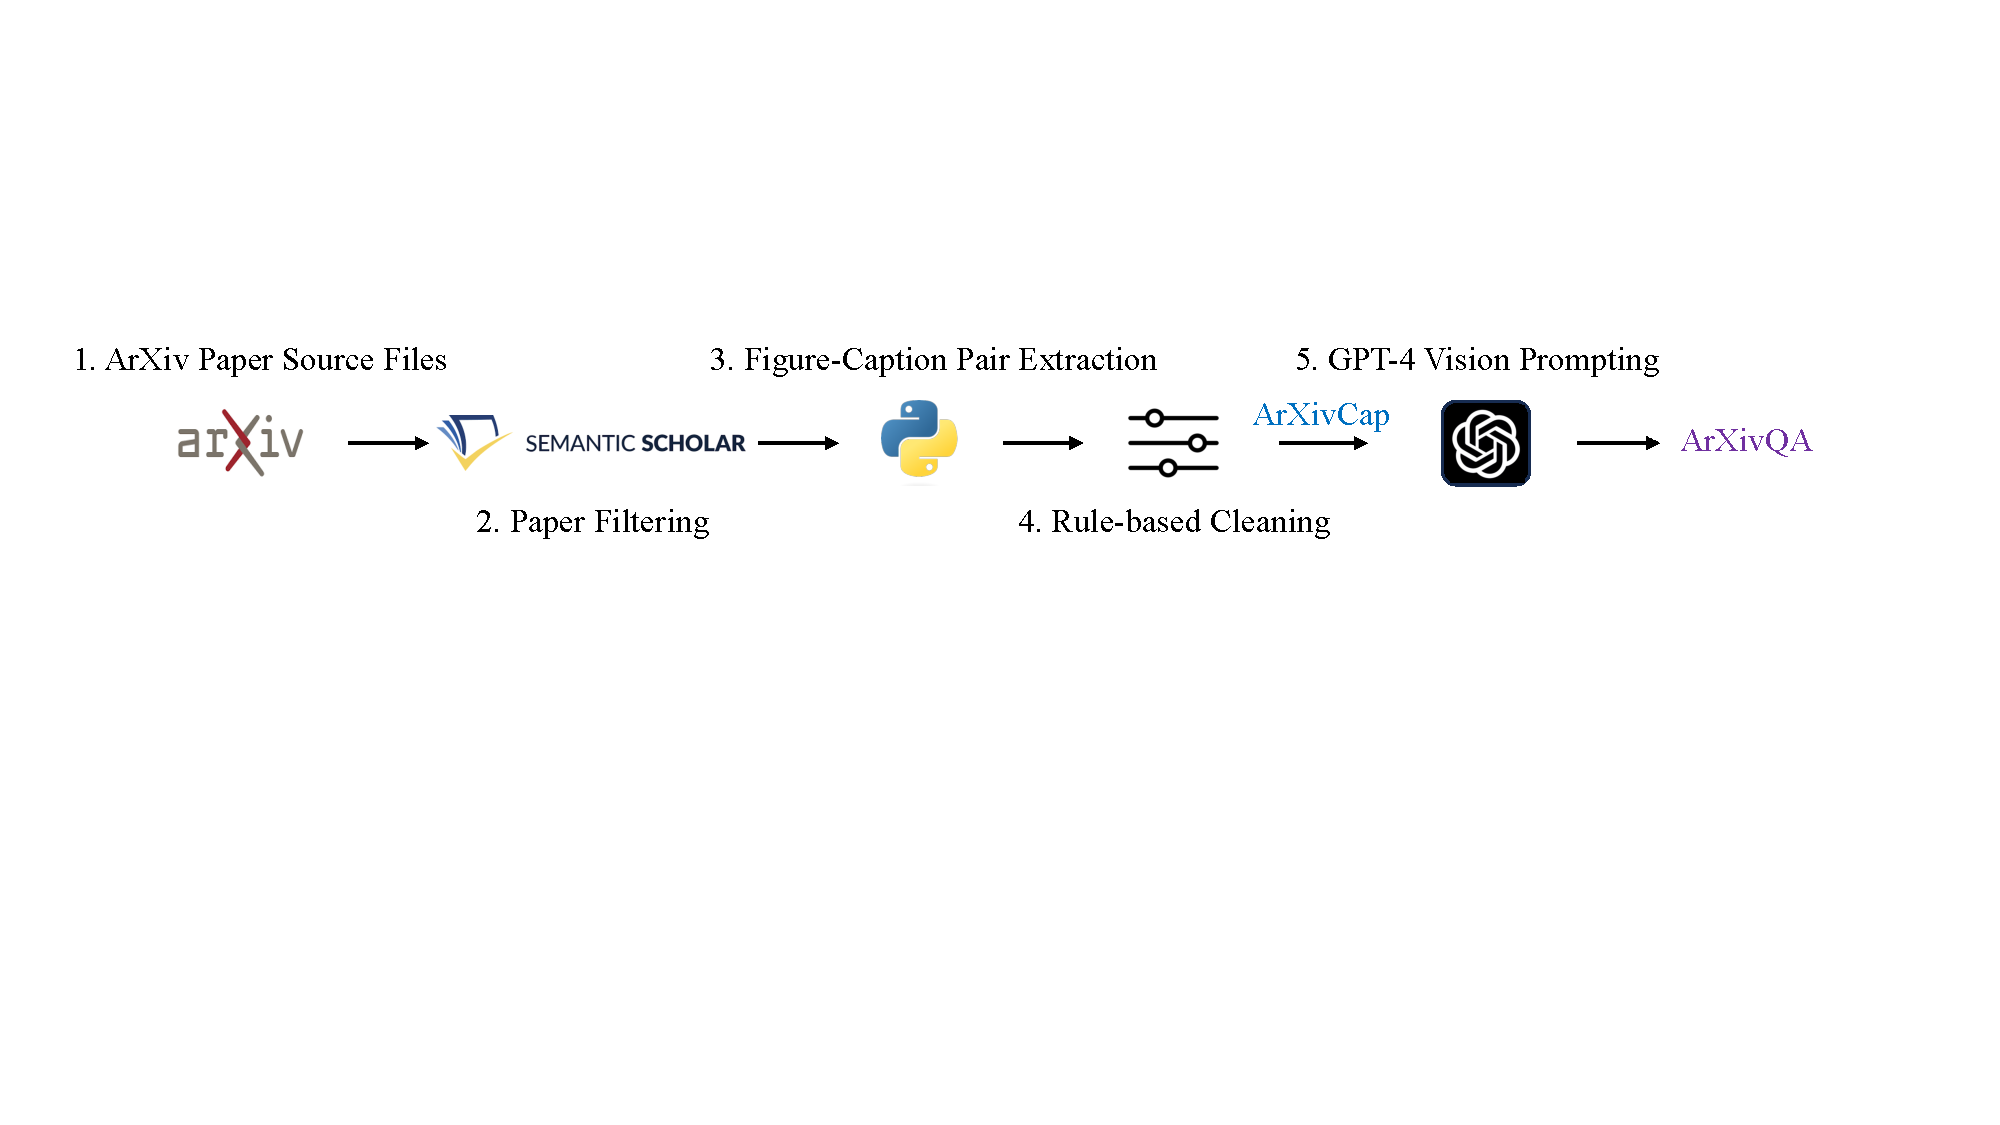
\includegraphics[width=0.95\linewidth]{figs/process.pdf}
    \caption{Overview of our dataset curation process. Starting from the ArXiv paper source files, we ensure the paper quality by selecting papers according to publication records. Figure and caption pairs are extracted and then cleaned according to manually designed rules. ArXivQA is generated by prompting GPT-4V with a curated template.}
    \label{fig:dataset-curation-process}
\end{figure*}


\subsection{ArXivCap}
\label{subsec:ArXivcap}

% \subsubsection{Construction Process of ArXivCap}
\paragraph{Construction Process} We outline the creation process of ArXivCap below and Figure~\ref{fig:dataset-curation-process} gives an overview.

\noindent\emph{Paper Filtering with Publication Type:}
\DatasetName is extracted from ArXiv~\cite{clement2019use}, which is under CC-0 licence for modification and distribution. 
% Therefore, we have the permission to create and distribute \DatasetName. 
% The files in the ArXiv dataset are in tar format, which includes LaTeX files and their corresponding image files. 
The raw files of papers posted on ArXiv tar files before June 2023 are downloaded. 
To ensure the quality of our dataset, we employ a rigorous selection process to filter potentially low-quality papers that might influence the figure-caption pair quality. 
Firstly, we retrieve meta-information for papers from Semantic Scholar~\cite{kinney2023semantic}, which contains the publication record for each paper. 
Papers with publication types \texttt{JournalArticle},  \texttt{Conference}, or \texttt{Review} are kept as we assume the peer-review process could ensure the overall figure-caption quality is satisfactory.
We further exclude papers with titles exceeding 100 words or abstracts longer than 300 words, in alignment with common submission requirements.
% We further filter out papers with titles longer than 100 words, or with an abstract longer than 300 words, according to common submission requirements.
% for examples. 
% There are 2,285,111 papers and 13,945,502 images in total till this step.


% % Use figure* for multi-column figure
\begin{figure}[!t]
    \centering
  \begin{subfigure}{0.45\textwidth}
    \centering
    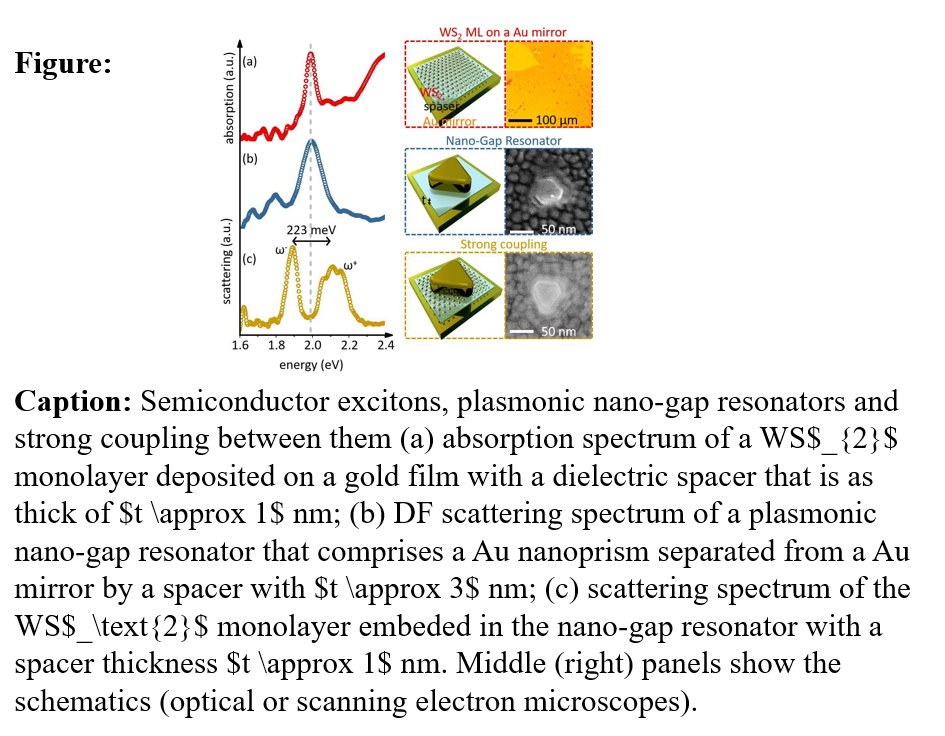
\includegraphics[width=\textwidth]{figs/examples/1-1.png}
    \caption{Single Figure-Caption}
    \label{fig:subfig1}
  \end{subfigure}
  \hfill
  \begin{subfigure}{0.45\textwidth}
    \centering
    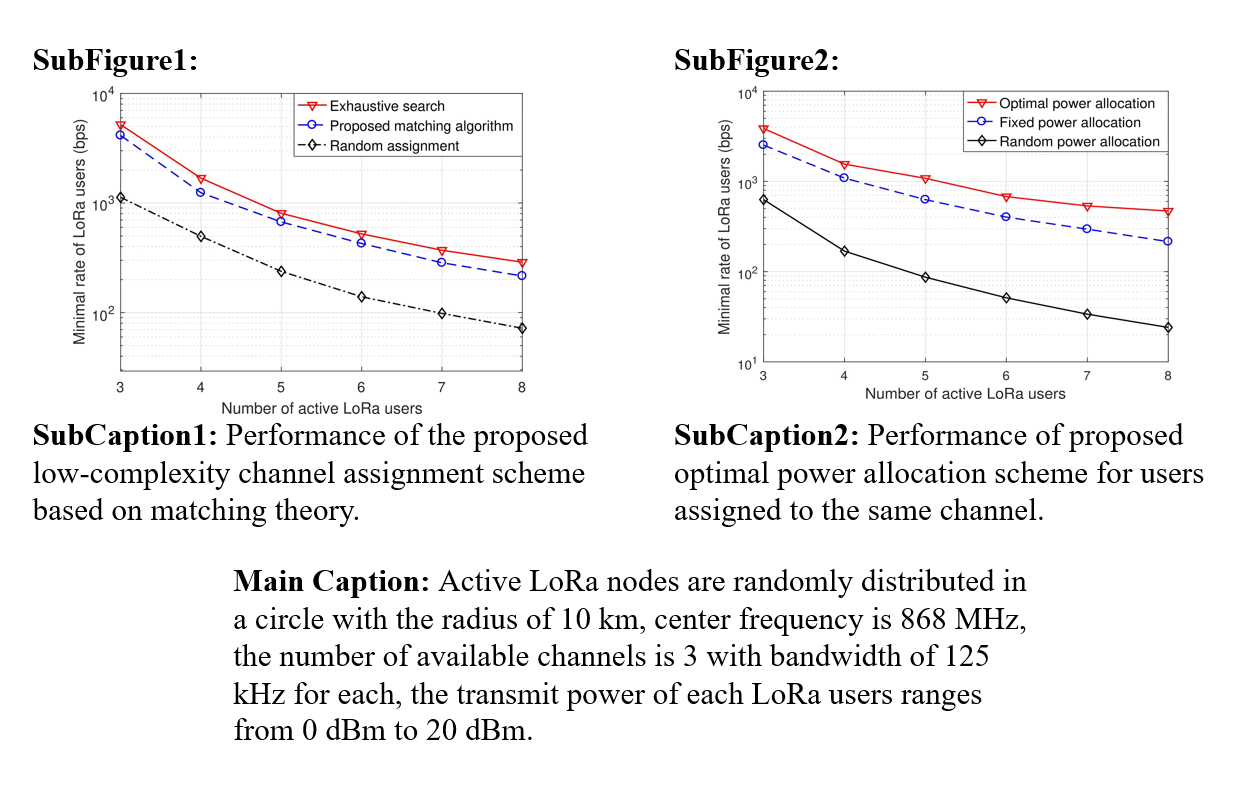
\includegraphics[width=\textwidth]{figs/examples/1-2.png}
    \caption{Multiple Figure-Caption}
    \label{fig:subfig2}
  \end{subfigure}
  \caption{Chunk Example. \lilei{add case of arxiv qa}}
  \label{fig:chunk_example}
\end{figure}

% \paragraph{Unify Image Format} 
% We utilize ImageMagisk~\cite{imagemagick} to convert images of various formats, including .ps, .epsi, .PS, .pdf, .PDF, .EPS, .eps, etc., into the JPEG format, while preserving the original jpg/jpeg and png images. ImageMagisk is a robust tool for image editing and transformation. Additionally, we standardize the output format to jpg/jpeg in RGB mode and remove the white border around images.

% according to our prior.
% This ensures that we include papers published in reputable journals, conference proceedings, or recognized review articles.
% We further keep papers satisfying the following requirements:
\noindent\emph{Figure-Caption Pair Extraction:}
Images and captions are extracted from the original LaTeX files by matching the syntax. 
We further use a robust tool ImageMagisk~\cite{imagemagick} to convert images into JPEG format for easy processing.
The extracted images and captions are stored in a designed chunk structure,
which consists of either a single figure-caption pair or multiple figures with their respective sub-captions and a main caption for the overall description.
This format is more consistent with the layout of academic papers, and
Figure~\ref{fig:chunk_example} illustrates the chunk structure.

% \begin{enumerate}% [leftmargin=2em]
%     \item The number of words in the abstract is in  $[10, 300]$.
%     \item The number of words in the title is in $[1, 100]$.
% \end{enumerate}

\begin{figure}[t!]
    \centering
    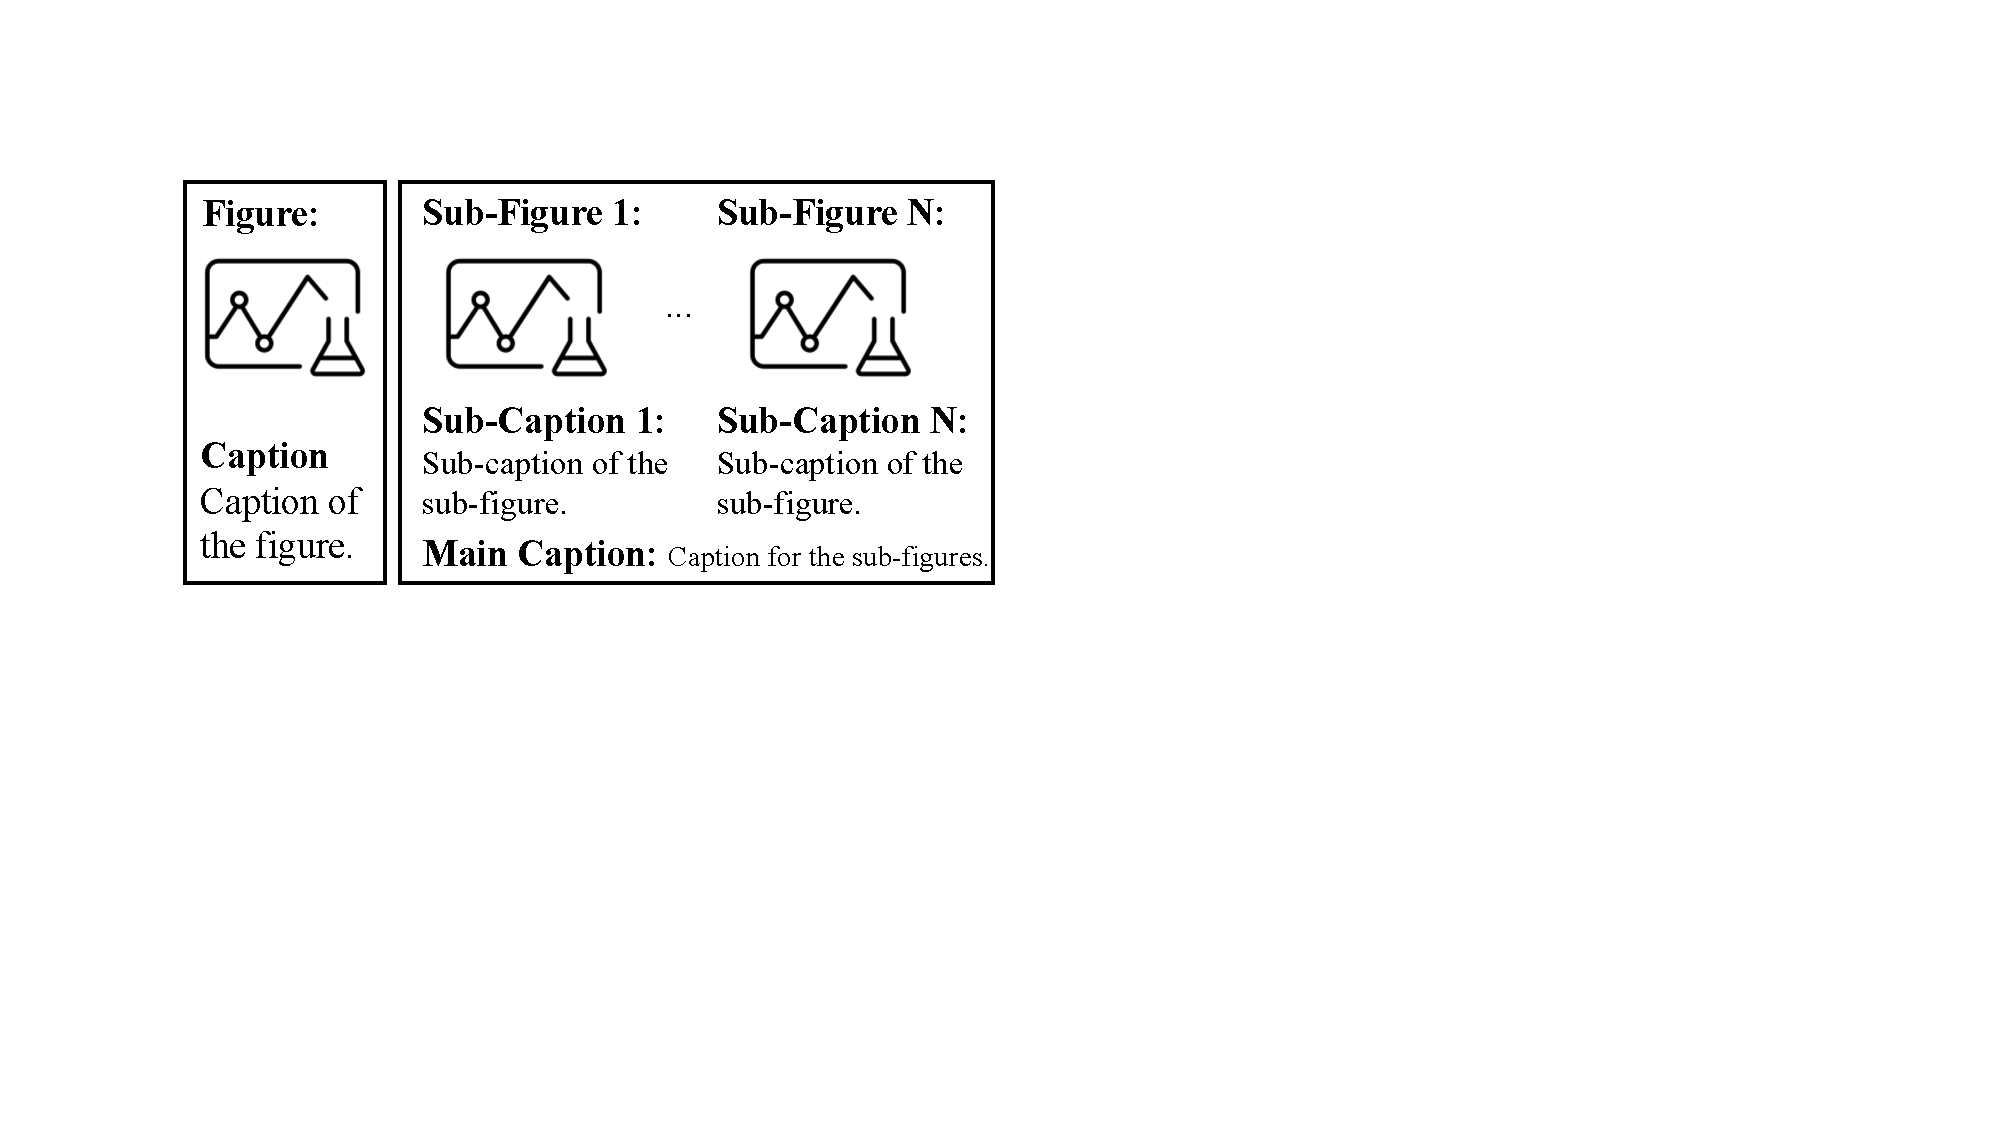
\includegraphics[width=0.9\linewidth]{figs/chunk-v2.pdf}
    \caption{Illustration of two types of figure-caption pairs. (Left) Single-Figure pair. (Right) Multiple-Figure caption pair has multiple sub-figures with corresponding sub-captions and an overall main caption. }
    \label{fig:chunk_example}
\end{figure}
% \paragraph{Filter Images}
% After resizing images using Lanczos resampling, we ensure that the maximum dimension of each image does not exceed 2016 pixels. Following a manual inspection of the images, we apply the following filters to refine the selection process further, retaining only the images that meet the specified requirements:

% \begin{enumerate}
%     \item The ratio between the width and height of the image is less than 100.
%     \item The width or height of the image is larger than 224 pixels.
%     \item The number of pixels in the image is less than 89,478,485.
% \end{enumerate}


\noindent\emph{Caption Cleaning and Image Filtering:}
After a manual inspection of the initially collected dataset, we design several transformations to clean the captions and filter the images.

\noindent\emph{Caption Cleaning}: (i) Chunks with captions shorter than 5 words are removed; (ii) For captions with LaTeX expressions such as math formulas and references, we apply the \texttt{pylatexenc}\footnote{https://github.com/phfaist/pylatexenc} to transform the LaTeX to text with math formulas retained, citations to a special symbol \texttt{<cit.>}, references to \texttt{<ref>}. An illustration of caption cleaning can be found in Appendix~\ref{apx:caption_clean}.
%\textgreater"


\noindent\emph{Image Filtering}: We remove images that are deemed to be problematic according to the following rules:
(i) Images with an aspect ratio larger than 100; (ii) Images with the shortest edge shorter than 224 pixels; and (iii) Images with pixel numbers larger than the decompression bombs threshold.
% The ratio between the width and height of the image is less than 100.
%     \item The width or height of the image is larger than 224 pixels.
%     \item The number of pixels in the image is less than 89,478,485.
% Replace incorrect newline characters with empty spaces.
    % \item Replace consecutive empty spaces with a single space.
    % Remove chunks that have captions with fewer than 5 words or no words at all.
   % Utilize pylatexenc to convert LaTeX to text, ensuring that math formulas are retained. Additionally, normalize citations and tables to "\textless ref \textgreater" and "\textless cit. \textgreater" format. (\cref{tab:pylatexenc_clean})
% \end{enumerate}

After these processes, 100 pairs are sampled to perform an additional manual inspection, where we found all of these pairs contained clear images and correct caption descriptions. We provide visualized figure-caption pairs in Appendix~\ref{apx:case_illustrations}.
\paragraph{Statistics of ArXivCap}
% In this section, we present a general analysis of \DatasetName. Detailed analysis can be found in the Appendix. 

% \begin{table*}[ht!]
    
%     \centering
    
%     \small 
%     \begin{tabular}{@{}lcccccc@{}}
%          \toprule
%         Field & Number & Total & Average & Minimum & Maximum & Quartile \\
%          \midrule
         
%         Title & 572,734 & 5,960,728 & 10.41 & 1 & 100 & (8, 10, 12) \\
                 
%         Abstract & 572,734 & 95,987,566 & 167.6 & 10 & 300 & (126, 165, 207) \\
        
%         Chunk Caption & 3,963,576 & 193,482,743 & 48.82 & 1 & 2,248 & (16, 36, 67) \\
        
%         Main Caption & 3,958,840 & 188,590,156 & 47.64 & 1 & 2,248 & (15, 35, 65) \\

%         Subcaption & 1,025,704 & 4,892,587 & 4.77 & 1 & 307 & (2, 3, 5) \\  

%         Images & 6,481,222 & N / A & N / A & N / A & N / A & N / A \\
%          \bottomrule
%     \end{tabular}
%     \caption{Word count statistics for title, abstract, captions and Image number. A word is defined as any sequence of characters matching the regular expression pattern r"\textbackslash w+". \cref{fig:chunk_example} shows the example of subcaption and main caption. The term "Chunk caption" encompasses all captions within it, including both the subcaption and the main caption contained within it.}
%     \label{tab:detail_statistic_title_abstract_image_caption}
% \end{table*}

\begin{table}[t!]
    \centering
    \resizebox{\linewidth}{!}{
    \begin{tabular}{@{}lccc@{}}
         \toprule
        Field & Number &  Average Len.  & Quartile of Len. \\
         \midrule
         
        Title & 572K &  10.4   & (8, 10, 12) \\ 
        Abstract & 572K &  167.6  & (126, 165, 207) \\
        \midrule 
        Main Caption & 3.9M  &  47.6 & (15, 35, 65) \\
        Subcaption & 1.0M  & 4.8 &  (2, 3, 5) \\  
        Chunk Caption & 3.9M &  48.8  & (16, 36, 67) \\
        \midrule 
        Images & 6.4M  & N / A  & N / A \\
         \bottomrule
    \end{tabular}}
    \caption{Word count statistics for title, abstract, captions, and Image number. 
    Chunk caption refers to the combination of subcaptions and the main caption for a multiple-figure case.}
    \label{tab:detail_statistic_title_abstract_image_caption}
\end{table}

\begin{table*}[ht!]
    \centering
\resizebox{\textwidth}{!}{
    \begin{tabular}{@{}lccccc@{}}
         \toprule
        Dataset & Image Number & Paper Number & Image Category & Domain & Real Data \\
         \midrule
                 FigCAP~\citep{chen2020figcap} & 219K & N / A & Bar, Line and Pie Charts & N / A & \xmark \\
        
         SciCap~\citep{Yang2023SciCap+} & 2.1M & 295K & Open-Category & Computer Science and Machine Learning & \cmark \\

         M-Paper~\citep{hu2023mplugpaperowl} & 350K & 48K & Open-Category & Mainly "Deep Learning" & \cmark \\   
        
         ArXivCap (Ours) & 6.4M & 572K & Open-Category & Open-Domain & \cmark \\
 
        \midrule 
FigureQA~\citep{kahou2017figureqa}  & 140K & N / A & Bar, Line and Pie Charts & N / A & \xmark \\
                 
        DVQA~\citep{kafle2018dvqa} & 300K & N / A & Bar Charts & N / A& \xmark \\
         ArXivQA (Ours) &  32K & 16.6K & Open-Category & Open-Domain & \cmark \\
         \bottomrule
    \end{tabular}}
    \caption{Comparison with previous scientific figure datasets. Our ArXivCap is the largest captioning dataset and our ArXivQA is the only QA dataset that covers a wide range of domains from real papers. }
    \label{tab:dataset_comparison_1}
\end{table*}

% \crossmark & \cmark 

Table~\ref{tab:detail_statistic_title_abstract_image_caption} lists the dataset statistics. 
ArXivCap consists of 572K papers, containing 6.4M high-quality images in total with 193M words. 
A word cloud illustration of captions can be found in the Appendix~\ref{apx:caption_word_cloud}.
Figure~\ref{fig:domain-distribution} demonstrates the paper domain distribution extracted from ArXiv, where we find that our ArXivCap covers 32 domains, such as computer science, mathematics, physics, and economics.
As shown in Table~\ref{tab:dataset_comparison_1}, compared with previous scientific figure datasets, our ArXivCap is the largest figure-caption dataset collected from real papers and covers a wide range of scientific domains, serving as a valuable resource for improving and benchmarking LVLMs.

%, and our ArXivQA is the only open-domain QA datasets with diverse figure types.

% , providing a comprehensive general knowledge for LVLMs.

% It is the largest image-caption dataset for academic figures, encompassing a diverse array of domains and image categories. \cref{tab:dataset_comparison_1} presents comparison between \DatasetName and other datasets.
 % We get the domain category for each paper from \cite{ArXiv.org_submitters_2023}. 



% \begin{table}[tbh!]
    \centering
    \begin{tabular}{l|c}
    \toprule
       Field  & Total Number \\
       \midrule
       Title \& Abstract & 572,734 \\ 
       Image & 6,481,222 \\ 
       Caption & 3,961,133 \\ 
       \bottomrule
    \end{tabular}
    \caption{Data Statistics of the curated dataset.}
    \label{tab:data_statistics}
\end{table}

\begin{table}[tbh!]
    \centering
    \begin{tabular}{l|cc}
    \toprule
       Field  & Total Number & Word Number \\
       \midrule
       Block Caption & 3,963,576 & 193,482,743 \\ 
       Main Caption in Block & 3,958,840 & 188,590,156 \\ 
       Subcaption in Block & 1,025,704 & 4,892,587 \\ 
       \bottomrule
    \end{tabular}
    \caption{Caption Statistics of the curated dataset.}
    \label{tab:caption_statistics}
\end{table}


% \begin{table}[tbh!]
%     \centering
%     \begin{tabular}{l|cc}
%     \toprule
%        Field  & Statistic \\
%        \midrule
%        Image Number & 6,481,222 \\ 
%        Total Size & 892GB \\ 
%        \bottomrule
%     \end{tabular}
%     \caption{Image Statistics of the curated dataset.}
%     \label{tab:image_statistics}
% \end{table}


% Use figure* for multi-column figure
\begin{figure}[t!]
    \centering
    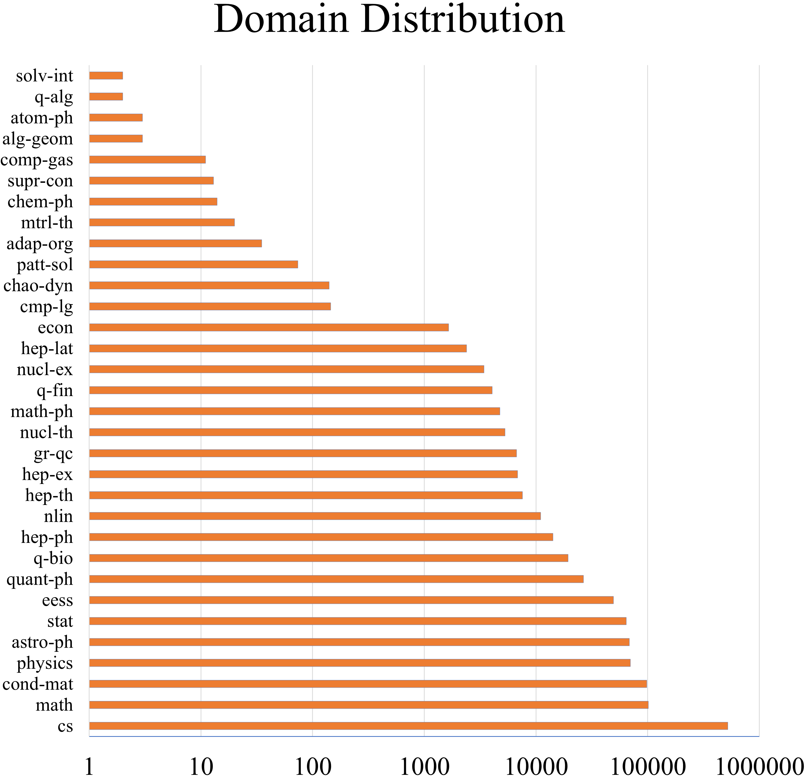
\includegraphics[width=0.9\linewidth]{figs/domain-distribution_500.png}
    \caption{Paper domain distribution of ArXivCap. See Table~\ref{tab:domain-full-name} in Appendix~\ref{apx:arxiv_cap} for the full name of each domain.}
    \label{fig:domain-distribution}
\end{figure}


\subsection{ArXivQA}
\label{subsec:arxiv_qa}
As our ArXivCap contains diverse images from scientific domains, we assume that learning to answer questions about these figures could boost scientific reasoning ability. Following the successful practice of LLaVA~\citep{liu2023llava}, we adopt GPT-4V to generate instruction-tuning datasets for generating the QA pairs based on the figures extracted from scientific papers.
Specifically, we design a prompting template to query GPT-4V for generating QA pairs based on 35K images randomly sampled from our ArXivCap.
Table~\ref{tab:prompt_for_ArXivqa} in Appendix~\ref{apx:prompt_template} provides the template we used for the prompt.
The generated pairs are parsed according to the format requirement and we discard the samples without options and rationales.
There are 100K QA pairs after filtering the invalid samples. 
The dataset comprises questions with an average word count of 16.98 for the question text.
% and options for the question with an average word count of 31.86. 
On average, there are 4.20 options per question and the average length of the text for a single option is 7.59 words.
Appendix~\ref{apx:case_illustrations} provides samples from the ArXivQA dataset.

As a preliminary study, we sample 1,000 samples from ArXivQA and prompt open-sourced LVLMs to predict answers given the questions and options. 
A simple prompt is designed to employ GPT-4 for extracting the answer label from the model generations.
For human performance, we ask four authors to perform predictions on a 100-sample subset (where 17 samples are from the CS domain). Each of them is asked to answer 50 samples and the accuracy scores are obtained by averaging two annotators.
As shown in Table~\ref{tab:arxiv_qa_acc}, most models struggle to perform satisfactorily on the ArXivQA dataset, falling far behind human performance. This verifies our premise that current open-sourced LVLMs fail to understand scientific figures. We also notice that simply increasing the model scale from 7B (LLaVa-1.5-7B) to 13B (LLaVa-1.5-13B) does not yield a significant boost, which indicates that the ability for multimodal mathematical reasoning cannot be simply acquired from the LLM-side only. 




\begin{table}[t!]
    \centering
    \small 
    \begin{tabular}{l|c}
        \toprule
        Model & Accuracy \\
        \midrule
        InstructBLIP-Vicuna7B & 7.0\% \\
        LLaVA-1.5-7B & 44.2\% \\
        LLaVA-1.5-13B & 46.8\% \\
        OpenFlamingo-9B & 9.9\% \\
        IDEFICS-Instruct-9B & 34.5\% \\
        Qwen-VL-Chat & 46.6\% \\
        \midrule 
        \textcolor{gray}{Human (100-sample Subset)} & \textcolor{gray}{80.0\%} \\
        \textcolor{gray}{Human (CS subset)} & \textcolor{gray}{88.2\%} \\
        \bottomrule
    \end{tabular}
    \caption{Evaluation results on the sampled 1,000 ArXivQA samples. }
    \label{tab:arxiv_qa_acc}
\end{table}
% Domain and Option Number, Option length, verb visualization?




\input{tables/ArXivqa}

\section{Experiments}

We conduct experiments to (i) validate the effectiveness of ArXivQA for boosting multimodal scientific reasoning for open-source LVLMs~(\S\ref{subsec:math_reasoning}) and (ii) benchmark LVLMs capability to comprehend scientific figures with ArXivCap~(\S\ref{subsec:exp_arxivcap}).


\subsection{Boosting LVLMs with ArXivQA}
\label{subsec:math_reasoning}

\subsubsection{Experimental Settings}
\label{subsubsec:exp_setting}
We adopt Qwen-VL-Chat-7B~\citep{Qwen-VL}
as the backbone due to its support for interleaved image-text input formats and high-resolution images.
We fine-tune it on our ArXivCap (Qwen-VL-Chat-7B$_\text{ArXivCap}$), ArXivQA (Qwen-VL-Chat-7B$_\text{ArXivQA}$) and combination of these two datasets (Qwen-VL-Chat-7B$_\text{ArXivCap + ArXivQA}$) for three epochs with a learning rate of 1e-5 following the original paper.
We combine the answer and the rationale in ArXivQA to form the target output during training. 
Models are evaluated on MathVista~\citep{mathvista}, a benchmark that requires fine-grained, deep visual understanding and compositional reasoning. MathVista contains 6,141 examples, consisting of five multimodal tasks Figure QA, Geometry Problem Solving, Math word problem, Text Book QA, and Visual QA. 
We select 478 multiple-choice questions in the \texttt{testmini} split to avoid the inconsistency of answer parsing. We compute the accuracy scores and adopt the provided prediction files for calculating the baseline performance.
% is adopted as the metric.

\subsubsection{Results}

As shown in Table~\ref{tab:mathvista_ret},
fine-tuning on our Multimodal ArXiv, especially on the ArXivQA dataset, consistently boosts the performance, helping the open-sourced Qwen-VL-Chat achieve a comparable overall MathVista reasoning performance.
Due to the wide coverage of the scientific figures, the performance gain mainly comes from significantly improved Geometry Problem Solving, Textbook QA, and Visual QA tasks. For example, after fine-tuning on the ArXivQA dataset, the accuracy is increased from 19.1\% to 34.0\% and from 46.7\% to 70.0\% on Geometry Problem Solving and Textbook QA tasks, respectively.
The improvement on Math Word Problem is marginal, where we think the domain-specific data augmentation can be further explored with a curated filtering dataset on our dataset~\citep{gao2023gllava}.
On the contrary,
the accuracy of Figure QA deteriorates slightly compared with the original backbone model, which we attribute to the fact that most of the plots in the Figure QA evaluation are sampled from synthesized datasets such as DVQA~\citep{kafle2018dvqa}, exhibiting great gaps between real-world paper figures.

\subsubsection{Analysis}
We investigate how different subject domains affect mathematical reasoning ability using pairs of questions and answers (QA). We focus on six domains with more than 5K samples each. From each domain, we randomly choose a subset of 5K samples to ensure fairness in comparison. We then fine-tune the Qwen-VL-Chat base model using QA pairs from each domain and observe how it affects the model's accuracy compared to its original state.
Figure~\ref{fig:domain_analysis} demonstrates the relative accuracy changes (i.e., $\frac{\text{Accuracy after Fine-tuning}}{\text{Original Accuracy}} - 1 $) after training the model on QA pairs from each domain. Our findings reveal several key points: (i) QA pairs from the Computer Science (CS) domain are highly effective for improving mathematical reasoning ability, achieving a notable 27.09\% relative improvement. We attribute this to the compositional nature of the CS area. (ii) The most beneficial domain varies depending on the specific task. For instance, QA pairs from astrophysics domains enhance geometry problem-solving, while those from Condensed Matter improve performance in math word problems. (iii) Most domains hurt the Figure QA task. This suggests that synthetic Figure QA might not be the best benchmark for assessing realistic reasoning ability.
These findings underscore the efficacy of generated QA pairs and offer valuable insights for future research, such as adjusting task-specific weights in the dataset accordingly.



\section{The CC-Layer}
\label{sec:implement}
\subsection{Constructing the CC-layer}
\label{sec:implement_construct}
Given a discrete feature map $\varbold{I}$ of shape $[N,C_{in},H,W]$, we are interested in a layer that produces $\varbold{I'}=CC\{\varbold{I}\}$ of shape $[N,C_{out},H',W']$ which is resized by a (non-integer) scale-factor $(s_h, s_w)$. Here $N$ is the batch-size, $C$ is the number of channels. $H,W$ are spatial dimensions. The desired spatial size $H',W'$ may be chosen at inference time.
Our CC-layer consists of 4 principled building blocks, marked by numbers in Fig.~\ref{fig:overview} (for simplicity, $I$ and $I'$ are drawn as 2D vectors in Fig.~\ref{fig:overview}, i.e.,  4D tensors with $N=1$ and $C=1$). These are described next:

\textbf{Block 1 -- Projected-grid:} 
The Projected grid \varbold{$\textbf{g}$} matches each output `pixel' $\textbf{n}$=$(i', j')$$\in$$I'$ to a sub-`pixel' location \varbold{$\textbf{g}_n$} in the continuous space of the \ben{input} $I$. This grid is captured by a tensor of shape $[2,H',W']$ where the the first dimension are the 2 projected sub-`pixel' coordinates (vertical and horizontal) of each output `pixel' $\textbf{n}$=$(i', j')$$\in$$I'$, and $H', W'$ are for all the output `pixels'.

%\michal{why don't we see the number of Fig.4 in the next paragraph?}

Let's start with a simple example. Fig.~\ref{fig:grid}.a depicts a standard 1D  downscaling by %an integer 
$2$. Note that even when the scale-factor $s$ is an integer (or an inverse integer: ${s=\ben{\nicefrac{1}{2}}}$ in this case), it is  \emph{wrong} to map an output `pixel' position $\textbf{n}$$\in$$I'$  to its input position in $I$ by simply multiplying (or dividing)  by the scale-factor $s$. It can be observed in Fig.~\ref{fig:grid}.a   that ${\varbold{\textbf{g}_n}\neq2\textbf{n}=\textbf{n}}/{s}$
%\ben{\nicefrac{\textbf{n}}{s}}}$.
To obtain the correct mapping, let's
define $d_{out}$  to be the distance of any output `pixel'  
%\textbf{n}$$\in$$I'$  
\michal{$\textbf{n}$}
from the leftmost boundary of $I'$.  $d_{out}$  is measured in units of output `pixels'. The matching coordinates \varbold{$\textbf{g}_n$}   in the \ben{input} $I$  is  defined to have a distance $d_{in}$ from the leftmost boundary of  $I$, and is measured in units of input `pixels'. The correct mapping rule across image scales~\cite{MATLAB:2010} is $d_{in}$=${d_{out}}/{s}$, 
since the total shape (from boundary-to-boundary) is resized, rather than discrete `pixel' centers. Since the first `pixel' \emph{center} (in any \ben{feature map/image}) is always half a `pixel' away from the leftmost boundary, hence:
%we can easily relate $d$ to $n$ and to $\varbold{\textbf{g}_n}$, by 
$d_{out}$=$n$+$\frac{1}{2}$  and  $d_{in}$=$\varbold{\textbf{g}_n}$+$\frac{1}{2}$.
%Plugging it in, we get the
This entails the
well known relation used in image resizing methods~\cite{MATLAB:2010}: 
%$ \varbold{\textbf{g}_n}$=$\frac{n}{s}$+$\frac{1}{2}$$\left(\frac{1}{s}-1\right)$
$ \varbold{\textbf{g}_n}$=$\frac{n}{s}$+$\frac{1}{2}$$(\frac{1}{s}$-$1).$

% \michal{the next paragraph is very tedious, can and SHOULD be shortened substantially.}
% However, we need to handle also non-integer output shapes. Such an example is illustrated in Fig.~\ref{fig:grid}.b. Since images or feature-maps  can only be represented  by integer-sized vectors/tensors, we will usually (but not always) determine the size of the output layer to be $out\_size =\lceil s \cdot in\_size \rceil$, However, the intrinsic (non-integer) output size $s \cdot in\_size$ must be kept, as this is the true size of the output, while the integer size contains an extra sub-`pixel' margin. Fig.~\ref{fig:grid}.b shows a projected grid for resizing a $4 \times 4$ input layer by 0.6 and 1.4,  respectively. The final output size ($3 \times 6$) is larger than the intrinsic size ($2.4 \times 5.6$), due to the ceiling $\lceil * \rceil$ operation. 
% % To prevent misalignments, we need to map each output `pixel' center to its correct input `pixel' center. For this we need to shift the output `pixels' by half of the margin $\textbf{n}=\textbf{n}' -(out\_size - in\_size \cdot s)/2$. Plugging this into the relation of $p$ to $p'$ we obtain:
% To prevent misalignments due to this added sub-`pixel' output margin, and guarantee that each output `pixel' center is mapped to its correct input location, we need to shift the output `pixels' by half of the added margin:  $\textbf{n}=\textbf{n}' -(out\_size - in\_size \cdot s)/2$. %Plugging this into the relation of $p$ to $p'$ we obtain:
% This yields the final accurate grid mapping:
However, we need to handle also non-integer output shapes. The intrinsic output size 
$s \cdot in\_size$ may not be an integer, yet images or feature-maps  can only be represented  by integer-sized vectors/tensors. We will usually (but not always) determine the size of the output $I'$ to be $out\_size =\lceil s \cdot in\_size \rceil$. Fig.~\ref{fig:grid}.b shows an example of a projected grid for resizing a $4 \times 4$ input \ben{feature map} by scales 0.6 and 1.4,  respectively. The final output size ($3 \times 6$) is larger than the intrinsic size ($2.4 \times 5.6$), due to the ceiling operation $\lceil$*$\rceil$.  Therefore, the final  grid mapping (which accurately covers all cases) is:
\begin{align}
    \varbold{g_n} = \frac{n}{s} + \frac{1}{2}\Big( in\_size - 1\Big) - \frac{1}{2s}\Big(out\_size-1\Big)    
    \label{eq:grid}
\end{align}
% Since every output `pixel', (i, j) is mapped to continuous 2D coordinates in the input feature-map, % Since the grid matches two location coordinates to each output `pixel', 
% it is a represented as a standard CNN tensor of order 4, with shape $[1,2,H',W']$, where 
% the batch size is 1. The second dimension is 2 for 2 spatial continuous coordinates in the input space and the last two are for the height and width of the output. 


% First we calculate a grid of sub-pixel coordinates, which matches output pixels locations in the input continuous space. Each output pixel is assigned to horizontal and vertical sub-pixel position in the input. This grid is a function purely of the scale-factors and the output shape. Thus, importantly, the grid can be determined at inference time dynamically.

% To accurately obtain the projected-grid, we need to acknowledge that discrete `pixels' have non-infinitesimal size, thus we distinguish between `pixel' ordinal numbers to continuous locations of their centers. Fig.~\ref{fig:grid}.a depicts a 1d standard downscaling by a factor of $\frac{1}{2}$. Note that it even when the downscalinfg/upscalingis by an integer scale-factor (2 in this case), it is wrong to map output `pixel' positions to input positions by directly multiplying by the scale-factor. We mark the discrete `pixel' coordinates by $p$ and the scale-factor by $s$. First we observe that $p' \neq sp$. In the figure it is clear that `pixel' 0 should not be mapped to output `pixel' 0, rather the boundary between `pixel' 0 to `pixel' 1. We define the distance from the left boundary as $d$ measured in units of full `pixel's. Since the first `pixel' center is half a `pixel' to the right with respect to the left boundary, $d=p+\frac{1}{2}$. To correctly resize, we need the total size of the input (4 in the example) to be mapped to the total size of the output, hence $d'=s \cdot d$. plugging in the relation between $p$ and $d$: $p'+\frac{1}{2} = s(p+\frac{1}{2})$ so that the mapping rule between input and output `pixels' is $p = \frac{p'}{s} + \frac{1}{2} \left( \frac{1}{s} - 1 \right)$.


% Next we need to handle non-integer output shapes. Since we can only represent images or feature-maps sizes as integers we will usually (but not always) determine the output size as $Ceil(s \cdot in\_size)$. However, the intrinsic size $s \cdot in\_size$ must be held. We point out that in some cases of resizing, it is crucial to specify both scale-factors and output shape. For example, in a sequence of resizing operations. Fig.~\ref{fig:grid}.b illustrates projected grid for resizing by 0.6 and 1.4 respectively. The final output size is thus bigger than the intrinsic size. Depending on the kernel support, the output can be influenced by `pixels' out of the image, thus padding policy is required. Any further operation conducted on the output feature-map should treat the intrinsic size and not the padded size. The most reasonable convention in such cases is to preserve the center of the feature-map so that it maps to the center of the output. For this we need to shift the output `pixels' by half of the margin $p'=p'' -(out\_size - in\_size \cdot s)/2$. To finally obtain the grid, we map integer output `pixel' locations to their projected sub-`pixel' location in the input, we get for each dimension with its own scale-factor, input shape and output shape: 
% \begin{align}
%     g_n = \frac{n}{s} + \frac{1}{2}\Big( in\_size - 1\Big) - \frac{1}{2s}\Big(out\_size-1\Big)    
%     \label{eq:grid}
% \end{align}
% Since every output `pixel', (i, j) is mapped to continuous 2D coordinates in the input feature-map, % Since the grid matches two location coordinates to each output `pixel', 
% it is a represented as a standard CNN tensor of order 4, with shape $[1,2,H',W']$, where 
% the batch size is 1. The second dimension is 2 for 2 spatial continuous coordinates in the input space and the last two are for the height and width of the output. 

\begin{figure}
%\vspace*{-0.5cm}
    \centering
    \hspace{-3cm}
    \begin{minipage}{.5\textwidth}
      \centering
      \hspace{1cm}
      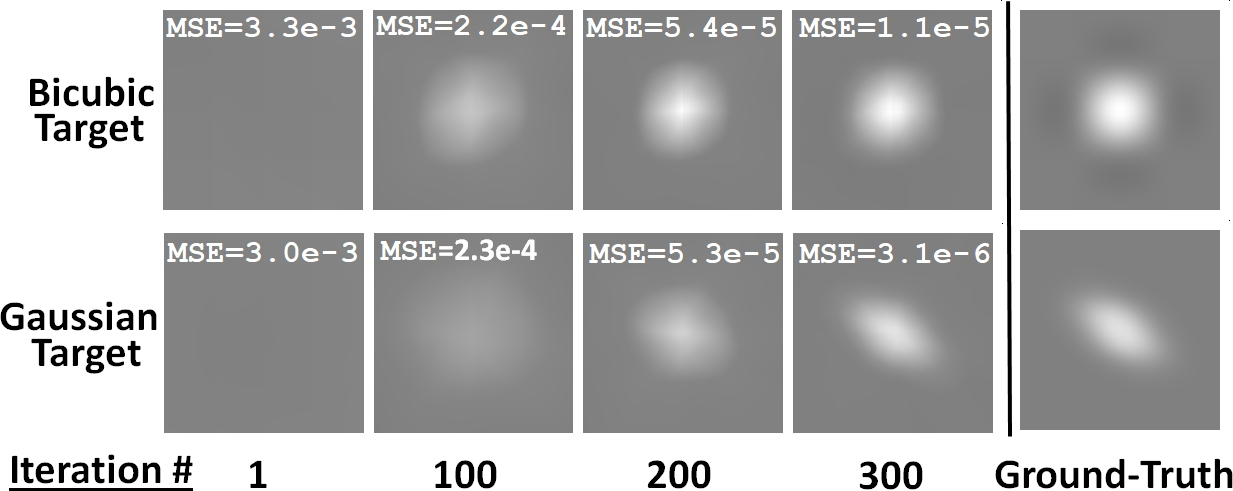
\includegraphics[width=1\textwidth]{figs/fig_visualize_Michal.jpg}
      \captionsetup{oneside, margin={-0.2cm,0cm}}
      \caption{\mbox{\it Visualizing the continuous learned kernels}}
      \label{fig:visualize}
    \end{minipage}
    \begin{minipage}{.4\textwidth}
        \vspace{-0cm}
        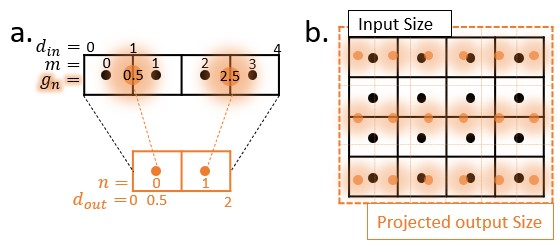
\includegraphics[width=1.5\textwidth]{figs/fig_grid.jpg}
        %\vspace*{0.5cm}
        \begin{minipage}{1.5\textwidth}
            \captionsetup{oneside, margin={1cm,0cm}}
            \caption{{\it The projected grid.}}
            \label{fig:grid}
         \end{minipage}%
    \end{minipage}%
    \vspace*{-0.5cm}
\end{figure}



\textbf{Block 2 -- Neighbors extraction:} For each grid point \varbold{$\textbf{g}_n$}, we now extract all its discrete nearest-neighbors $\varbold{\mathcal{N}[\textbf{n}]}$ \ben{from} $I$. These are all the input `pixels' centers within the support of the continuous kernel $\mathcal{K}_\theta$. This information is captured by a tensor of order 6 (blue tensor in Fig.~\ref{fig:overview}),  with shape $[N,1,C_{in},K,H',W']$ where K is the number of discrete neighbors in the kernel support. The second singleton dimension is for convenience in the next steps. We further need to extract the distances of each sub-`pixel' grid point \varbold{$\textbf{g}_n$} (of an output `pixel' {$\textbf{n}$}),  to all its discrete neighbors  ${\textbf{m}}\in I$. These distances $\varbold{\mathcal{D}[\textbf{n,m}]}$ are kept in a tensor $\varbold{\mathcal{D}}$ (shown in cyan in Fig.~\ref{fig:overview}), whose shape is $[K,2,H',W']$.

% Given a standard CNN input Tensor with dimensions Batch-size, Channels, Height and Width: $[N,C_{in},H,W]$.  We predefine support size (not necessarily an integer) for the continuous kernel $\mathcal{K}_\theata$. For each projected-grid point $\textbf{g'}$ we extract both values and distances to all input `pixels' within the kernel support. This stage produces a tensor consisting of all the neighbors values for each output `pixel'. This forces us to add a fifth dimension to the Neighbors tensor- the neighbors dimension. We actually extend this tensor to have 6 dimensions for convenience in the next stage, so the final shape is $[N,1,C_{in},K,H',W']$ where K is the number of neighbors in the kernel support. The Tensor of distances is shaped as a standard 2d CNN tensor, Its dimensions are: $[K,2,H',W']$. We use the batch dimension to distinguish between different neighbors. The second (channel) dimension is 2 to describe horizontal and vertical distances. Note that for simplicity, Fig.~\ref{fig:overview} depicts a case where $N=1, C_{in}=1$ and only the three last dimensions of the tensor are apparent.

% \textbf{Stage 3- Calculate weights:} The weights $\varbold{\mathcal{W}}$ are produced by the learnable model $\varbold{\mathcal{K}_\theta}$ applied to the distances tensor $\varbold{\mathcal{D}}$. 
\textbf{Block 3 -- Calculate weights:} The weights are produced by a learnable model $\varbold{\mathcal{K}_\theta}$, which is applied to the distances tensor:
%$\varbold{\mathcal{D}}$:
$\varbold{\mathcal{W} = \mathcal{K}_\theta \big\{ \mathcal{D}\big\}}$ (similarly to \cite{wang2018deep}).
A weight is assigned to connect between each output `pixel' and all its discrete input neighbors. Therefore, the weight tensor $\varbold{\mathcal{W}}$ will have a shape of $[1,C_{out},C_{in},K,H',W']$ 
(red tensor in Fig.~\ref{fig:overview}). 
%This tensor is marked in red in Fig.~\ref{fig:overview}. 
Its first singleton dimension is needed to match the size of the Neighbors tensor $\varbold{\mathcal{N}}$. As in standard conv, each output channel  $C_{out}$ is connected to all input channels $C_{in}$ through $\varbold{\mathcal{W}}$. We use a small neural network for $\varbold{\mathcal{K}_\theta}$ called the ``Internal-Net'' (marked in green in Fig.~\ref{fig:overview}). It is a simple CNN sequence of 1$\times$1 conv layers and ReLUs. This way every output `pixel' $\textbf{n}$ connects only to distances $\varbold{\mathcal{D}[\textbf{n}]}$ within its own set of discrete input neighbors. 

% The weights are produced by a learnable model which maps the distances calculated at stage 2 to corresponding weights for all the neighbors. This enforces consistency alongside expressivity. While each output `pixel' is calculated using a distinct local discrete kernel, all these local kernels are governed by the same underlying mapping function. We can choose to use a predefined fixed mapping, but we will usually use a learnable neural network, referred to as the internal-net. The input will be the distances tensor from preious stage. since we force the same mapping function to each output `pixel' we use several 1$\times$1 convolution layers and ReLUs in the internal-net. Consistency of the mapping to different neighbors is also enforced, since different neighbors are different instances in a batch. However, any model can be plugged to calculate the weights. Like in standard discrete convolutions, we have a set of continuous kernels, each maps all the input channels to an output channel. The weighted sum is actually taken not only over the neighbor values, but also over the input channels. Similarly to the neighbors tensor, the final weights tensor is of order 6: $[1,C_{out},C_{in},K,H',W']$ where the first dimension is the batch dimension which is always 1, to match the neighbors tensor.

\textbf{Block 4 -- Apply weights:} The final stage executes Eq.~\ref{eq:underlying} for the entire output tensor,
by multiplying the Weights tensor (red) with the Neighbors tensor (blue) and summing over all neighbors and input channels:
%. We simply multiply the Weights tensor (red) with the Neighbors tensor (blue) and sum over all the neighbors and input channels:
% For a given input feature-map $I$ of size $[N,C_{in},H,W]$, scale-factors $s_h, s_w$ and wanted shape $H',W'$ given at inference we finally get: 
\vspace*{-0.4cm}
\begin{align}
\varbold{I'}=
CC\{\varbold{I}\}= \sum_{c_{in}, k} \varbold{\mathcal{N}} \otimes \varbold{\mathcal{W}}
\end{align} 
with the following tensor shapes: 

$ \varbold{I'}:[N,C_{out},H',W'], \quad \varbold{\mathcal{N}}: [N,1,C_{in},K,H',W'], \quad \varbold{\mathcal{W}}:[1,C_{out},C_{in},K,H',W'] $

\subsection{Training and Generalization}
\label{sec:train}
CC is end-to-end trainable. The only trainable parameters of CC are $\varbold{\theta}$,  the parameters of $\varbold{\mathcal{K}_\theta}$. The gradient is propagated from the CC output through the weights tensor $\varbold{\mathcal{W}}$ to them. Gradients need to also be propagated to previous layers through the CC input. This is done easily through the neighbors extraction since it is just slicing (each neighbour neuron is actually a copy of an input neuron).

The output shape is determined by the shape of the grid $\varbold{{g}}$. Since $\varbold{\mathcal{K}_\theta}$ is a fully convolutional network, it can be applied to any spatial input size both at training and inference. This means that regardless of what sizes and scales we train on, a single CC, with a single set of parameters $\varbold{\theta}$ is applicable to any size and scale determined at real-time.

The input to  $\varbold{\mathcal{K}_\theta}$ is 
$\varbold{\mathcal{D}}$, which through the grid  $\varbold{{g}}$ depends only on the desired output scale \&
shape. Naturally, to generalize to many scales, we can sample various scales during training. However, being fully 1$\times$1 convolutional, $\varbold{\mathcal{K}_\theta}$ actually maps every 2D distance vector
%distance (two coordinates -- vertical and horizontal)
$\varbold{\mathcal{D}[\textbf{n,m}]}$ to a single value (weight) $\varbold{\mathcal{W}[\textbf{n,m}]}$. This means that $\varbold{\mathcal{D}}$ actually contains a huge batch of
inputs. This produces an interesting advantage: in almost all cases CC generalizes from one scale to any other scale. This happens as long as the diversity of distances in a single grid is reasonable. Eq.~\ref{eq:grid} suggests that if the scale is a rational number with a small numerator, 
then there exists only a small set of grid coordinates, and consequently a small set of unique distances $\varbold{\mathcal{D}[\textbf{n,m}]}$. For example, for $s=\nicefrac{1}{2}$ and a kernel with support of 2$\times$2, we get:
%\rightarrow 
$\varbold{\mathcal{D}[\textbf{n}]} = \Big\{(-\nicefrac{1}{2},-\nicefrac{1}{2}), 
(-\nicefrac{1}{2},\nicefrac{1}{2}), 
(\nicefrac{1}{2},-\nicefrac{1}{2}), 
(\nicefrac{1}{2},\nicefrac{1}{2})
\Big\} \ \ \varbold{\forall \textbf{n}}$, which will not generalize to other scales/distances. In other words, generalization occurs over the distribution of distances $\varbold{\mathcal{D}}$  between the grid points and `pixel' centers. If this distribution collapses to a small set of possibilities, then such generalization is damaged. However, training with a \emph{randomly} selected float scale-factor will give a huge diversity of sub-`pixel' distances in $\varbold{\mathcal{D}}$, hence will be able to generalize with very high probability to any other scale factor.
%\michal{Is this still true for large gaps between the train-scale  and the test-scale? After all, this will lead to a large difference in support size of K}. \assaf{supprt size of K is independent of the scale} 
Empirical evaluation of this property is described in the experiments section and in Fig.~\ref{fig:generalize}.
%\michal{Reference to Fig. 7 broken}
% \textbf{Cross-scale generalization:} Since the learning model $\mathcal{K}_\theta$ is unaware of the scale, it can be trained to one scale and generalize to another, under reasonable conditions. the scale trained on, cannot be a special case that collapses back to convolution, or a rational number with a denominator that is too small. In other words, generalization occurs over the distribution of distances between the grid and `pixel' centers. If this distribution collapses to a small set of possibilities then such generalization is damaged. A randomly selected float scale-factor will be able to generalize with probability ~1. 


% \textcolor{red}{
% \subsection{Training the CC-layer for dynamic scale generalization}
% \begin{itemize}[leftmargin=0.7cm]
% \item Please explain how to train the CC-layer so that it can generalize at test-time to any desired scale and shape.
% \item Please stress that although we use many scale/shape augmentations of the output layer, this is still a single trained network (as opposed to training multiple different networks, each for a different fixed output scale/shape). This is obvious to us, but may be a natural misconception of the reviewers, so it is worth stressing. Better safe than sorry...
% \end{itemize}
% }
\subsubsection{Experimental Settings}
\label{subsubsec:arxiv_cap_setting}




\paragraph{Dataset}
We divide ArXivCap into training and test sets with a 9:1 ratio for evaluation. The test set includes:
161.3K samples for single-figure captioning,
12.8K samples for multiple-figure captioning,
57.2K samples for contextualized captioning, and
57.2K samples for title generation.

\paragraph{Evaluated Models}
We select various LVLMs covering different architectures. 
(1) LVLMs designed for dealing with a single image, BLIP2-OPT-6.7B~\citep{li2023blip2}
, InstructBLIP-Vicuna7B~\citep{dai2023instructblip}, 
% MiniGPT4~\citep{zhu2023minigpt4}, 
LLaVA-1.5-7B/13B~\citep{liu2023llava15}. Due to the ability limitation, we only benchmark these models on the single image captioning task;
(2) LVLMs capable of handling interleaved text-image inputs, such as OpenFlamingo-9B~\citep{Alayrac2022FlamingoAV,awadalla2023openflamingo}, IDEFICS-Instruct-9B~\citep{laurencon2023obelics}, Qwen-VL-Chat-7B~\citep{Qwen-VL}. These models are evaluated on all the tasks we proposed;
(3) Proprietary models such as Gemini 1.0 Pro Vision and GPT-4V.
Due to the large scale of our test set, we randomly sample a subset consisting of 500 instances for evaluating these two models to reduce costs, with corresponding scores colored in \textcolor{gray}{grey}. Details of evaluated models and the task prompts used are provided in Appendix~\ref{apx:evaluation_details}.

\paragraph{Training Settings} 
To investigate whether in-domain training can enhance the model's capabilities, we train the Qwen-VL-Chat-7B on ArXivCap using the same setting as in \S\ref{subsubsec:exp_setting}. To fit the input length limit, we set the maximum number of figures per sample to four. The training process takes 70 hours with 8 NVIDIA A100s.
% To investigate whether in-domain training can enhance the model's ability, we train the Qwen-VL-Chat-7B for three epochs and adopt the AdamW optimizer~\citep{adam} with a learning rate of 1e-5 and weight decay set to 0.05, following the original setup of Qwen-VL-Chat.
% The dataset is split in a 9:1 ratio into training and test sets.
% We set the maximum figure number in a sample to $4$ to fit the input length limit.
% The training costs 70 hours with 8 NVIDIA A100 GPUs.

\paragraph{Metrics}BLEU-2~\citep{bleu}, ROUGE-L~\citep{lin-2004-rouge} and BERT-Score~\citep{bertscore} are adopted as the automatic evaluation metrics.
% We adopted BLEU-2 \citep{bleu}, ROUGE-L \citep{lin-2004-rouge}, and BERT-Score \citep{bertscore} as our automatic evaluation metrics. 
We also explore using GPT-4 to assist in caption evaluation. Our findings in Appendix \ref{apx:gpt4_eval} indicate that ROUGE-L and BLEU-2 scores are highly correlated with GPT-4's annotations. We primarily use these three metrics due to their convenience. A manual error analysis is conducted to supplement the automatic metrics~(\S\ref{subsubsec:manual_eval}).


% We also explore using GPT-4 to aid caption evaluation. Our results in Appendix~\ref{apx:gpt4_eval} show that ROUGE-L and BLEU-2 are highly correlated with the score annotated by GPT-4. We mainly use previous three metrics due to their convinence.
% Besides, a manual error analysis is performed to supplement the automatic evaluation (\S\ref{subsubsec:manual_eval}).
% As the automatic metrics cannot faithfully reflect the generation quality, we randomly sample pairs and perform human evaluation. We also incorporate GPT-4V for evaluation.


\begin{figure}[t!]
    \centering
    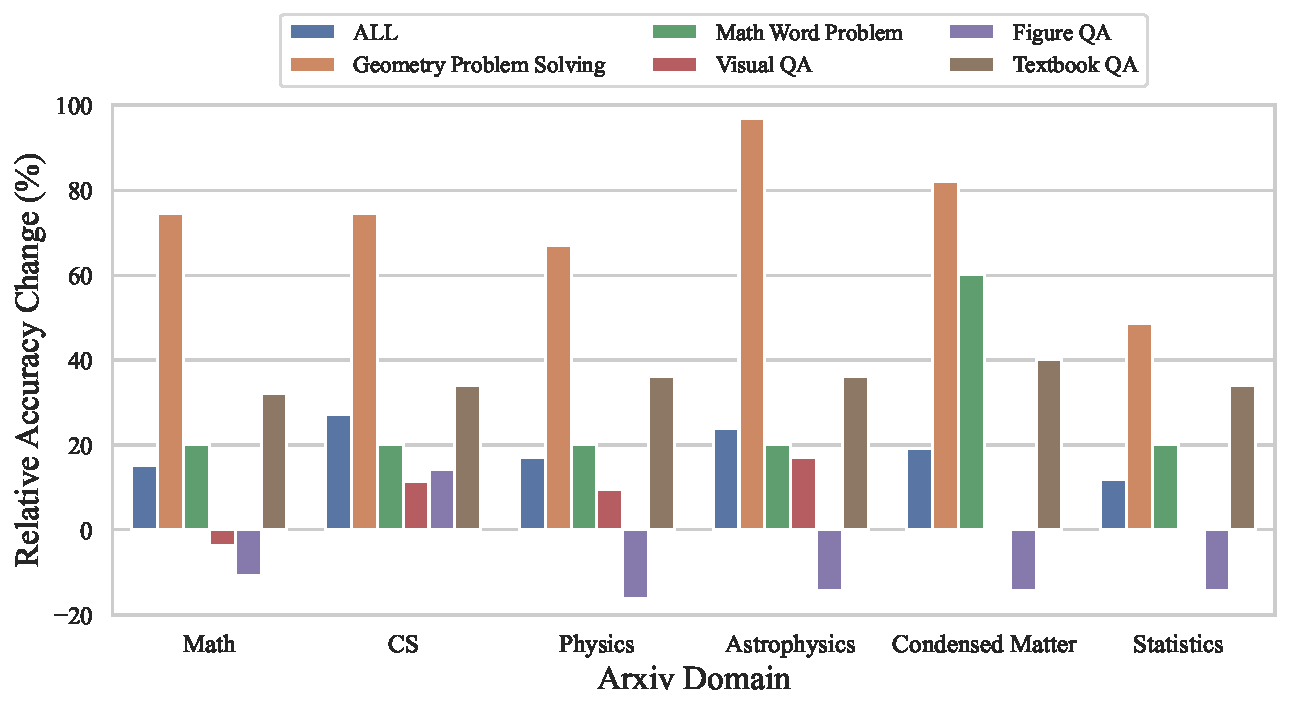
\includegraphics[width=\linewidth]{figs/domain_performance.pdf}
    \caption{Relative accuracy changes brought by the training on different domain ArXivQA samples.}
    \label{fig:domain_analysis}
\end{figure}
\begin{table}[t!]
    \centering
    \resizebox{\linewidth}{!}{
    \begin{tabular}{@{}l|ccc@{}}
    \toprule
    \textbf{Model}     &  BLEU-2 & ROUGE-L & BERT-S\\
    \midrule 
    % MiniGPT4 & & & \\ 
     BLIP-2-OPT-6.7B    & 2.1 & 7.1 & 81.1 \\ 
     InstructBLIP-Vicuna7B  & 3.7& 10.1 & 83.3 \\ 
     LLaVA-v1.5-7B    & 2.3 & 10.6 & 83.0 \\ 
     LLaVA-v1.5-13B    &2.6  & 10.7&  83.3 \\ 
      \midrule 
     OpenFlamingo-9B    & 5.7 &  9.9 & 82.4  \\ 
     IDEFICS-Instruct-9B & 2.5 & 9.1 & 83.5 \\ 
     Qwen-VL-Chat-7B &4.4 &11.1 & 81.8\\ 
     % + Title & & & \\ 
     % + Title and Abstract & & & \\ 
    Qwen-VL-Chat-7B$_\text{ArXivCap}$ & \textbf{8.9} & \textbf{15.8} & \textbf{83.3} \\ 
     % + Title & & & \\ 
     % + Title and Abstract & & & \\      
     \midrule
     % \textcolor{gray}{Bard} & \textcolor{gray}{3.4} & \textcolor{gray}{12.2} & \textcolor{gray}{82.2}\\ 
     \textcolor{gray}{Gemini 1.0 Pro Vision} & \textcolor{gray}{5.6} & \textcolor{gray}{14.5} & \textcolor{gray}{82.2}\\ 
     
        % \textcolor{gray}{GPT-4V} & \textcolor{gray}{5.7} &\textcolor{gray} {14.6}  & \textcolor{gray}{83.2}\\  200 subset 
      \textcolor{gray}{GPT-4V} & \textcolor{gray}{5.5} &\textcolor{gray} {14.2}  & \textcolor{gray}{83.3}\\  % 500 subset    
     \bottomrule
    \end{tabular}}
    \caption{Evaluation results of single figure captioning. \textcolor{gray}{Grey} results are obtained from a 500-sample subset. Despite most LVLMs struggle to produce high-quality captions of scientific figures, training with ArXivCap significantly boosts the performance.}
    \label{tab:single_cap_ret}
\end{table}
\begin{table}[t!]
    \centering
    \resizebox{\linewidth}{!}{
    \begin{tabular}{@{}l|ccc@{}}
    \toprule
    \textbf{Model}     &  BLEU-2 & ROUGE-L & BERT-S\\
    \midrule 
     Qwen-VL-Chat-7B &4.4 &11.1 & 81.8\\ 
      \quad + Title &5.7	&13.1&	81.6 \\ 
      \quad + Title and Abstract 	 & 6.0	 & 12.7	 & 81.4 \\ 
     \midrule 
    Qwen-VL-Chat-7B$_\text{ArXivCap}$ & 8.9 & 15.8 & 83.3 \\ 
     \quad + Title & \textbf{12.9}&	\textbf{18.6}	& \textbf{83.8} \\ 
      \quad + Title and Abstract &	12.7&	18.5&	83.8   \\      
     \bottomrule
    \end{tabular}}
    \caption{Evaluation results of single figure captioning with paper meta information.}
    \label{tab:cap_with_meta_ret}
\end{table}
\begin{table*}[tbh!]
\small 
\centering
\resizebox{\linewidth}{!}{
\begin{tabular}{@{}l|ccc|ccc|ccc@{}}
\toprule
\multirow{2}{*}{\textbf{Model}} & 
\multicolumn{3}{c}{\textbf{Multiple-Figure Captioning}}  & \multicolumn{3}{c}{\textbf{Contextualized Captioning}} & \multicolumn{3}{c}{\textbf{Title Generation}} \\
                       & BLEU-2 & ROUGE-L & BERT-S & BLEU-2 & ROUGE-L & BERT-S & BLEU-2 & ROUGE-L & BERT-S \\

% \midrule
% LLaVA-1          &      &       &            &      &       &            &      &       &            \\
% LLaVA-1.5       &      &       &            &      &       &            &      &       &            \\
% BLIP-2     &      &       &            &      &       &            &      &       &        \\
% InstructBLIP     &   0.0   &   10.1    &            &      &       &            &      &       &        \\
\midrule 
OpenFlamingo-9B  &     3.7  &  11.3     &  81.9           &    20.0  &     20.5  &         83.7  &    2.7   &   17.7    &  82.7      \\
IDEFICS-Instruct-9B &   3.6   & 10.8      &   82.8         & \textbf{20.7}   &     \textbf{22.6}  &     \textbf{85.7}        &    3.5    &     18.4 &     85.8    \\

Qwen-VL-Chat-7B   & 3.0     & 7.2   &  79.7          & 17.0   &   22.1  &  85.0         &  2.6    &     15.8  &   85.1         \\
 Qwen-VL-Chat-7B$_\text{ArXivCap}$ &  \textbf{10.6}     & \textbf{18.0}      & \textbf{83.6}           &    16.1    &    21.2     &        84.8     &     \textbf{6.7} &   \textbf{23.5}    & \textbf{86.8}      \\
\midrule
\textcolor{gray}{Gemini 1.0 Pro Vision}   &  \textcolor{gray}{6.1}    &   \textcolor{gray}{16.2}   &   \textcolor{gray}{83.1}     &  \textcolor{gray}{10.2}     &  \textcolor{gray}{20.2}       & \textcolor{gray}{84.5}           &   \textcolor{gray}{5.7}   &   \textcolor{gray}{21.8}  & \textcolor{gray}{85.9}     \\
\textcolor{gray}{GPT-4V}  &  \textcolor{gray}{5.7}   &  \textcolor{gray}{14.7}    &   \textcolor{gray}{83.0}         &    \textcolor{gray}{9.6}  &\textcolor{gray}{20.1}       & \textcolor{gray}{84.7}          &   \textcolor{gray}{4.0}   &   \textcolor{gray}{20.2}  &   \textcolor{gray}{86.0}     \\
% \textcolor{gray}{Bard}  &      &       &            &      &       &            &      &       &        \\
\bottomrule
\end{tabular}
}
\caption{Evaluation results of three newly defined tasks. The best results are highlighted in \textbf{bold}.}
\label{tab:ret_three_tasks}
\end{table*}
\subsubsection{Results}
\paragraph{Results of Single-Figure Captioning}
The evaluation results for the single-figure captioning task are presented in Table \ref{tab:single_cap_ret}. Despite achieving near-perfect performance on conventional image captioning tasks like MSCOCO \citep{lin2014mscoco}, open-source LVLMs, such as LLaVA models, face challenges when applied to academic figures. 
% Among the LVLMs, Qwen-VL-Chat emerges as the top-performing open-source candidate, surpassing its counterparts. 
For closed models, GPT-4V performs comparably with Gemini 1.0 Pro Vision.
Furthermore, continuous training on our dataset yields a significant performance boost for this task. For instance, fine-tuning results in a notable increase in the BLEU-2 score from 4.4 to 8.9, indicating a promising avenue for enhancing academic figure comprehension through domain-specific training.
We also investigate whether providing additional context information, such as the paper title and abstract, could help models generate better figure captions. As shown in Table \ref{tab:cap_with_meta_ret}, adding the title is beneficial evidenced by the boosted scores, while providing abstracts brings negligible gains.

% The evaluation results for the single figure captioning task are presented in Table~\ref{tab:single_cap_ret}. 
% Despite achieving almost perfect performance on conventional image captioning tasks such as MSCOCO~\citep{lin2014mscoco}, LVLMs encounter challenges when applied to academic figures. Among LVLMs, Qwen-VL-Chat emerges as the top-performing open-source candidate, surpassing its counterparts. 
% GPT-4V performs comparably with the Gemini 1.0 Pro. 
% Moreover, continuous training on our dataset yields a significant performance boost for this task. For instance, fine-tuning results in a notable increase in the BLEU-2 score from 4.4 to 8.9, indicating a promising avenue for enhancing academic figure comprehension through domain-specific training.
% We further investigate whether providing additional context information such as paper title and abstract could help models caption figures better.
% As shown in Table~\ref{tab:cap_with_meta_ret}, adding the title is beneficial for generating better captions while providing abstracts seems to bring negligible gains.

\paragraph{Results of Multiple-Figure Captioning}
As shown in the first block of Table \ref{tab:ret_three_tasks}, similar to single-figure captioning, multiple-image captioning poses a challenge for current open-source LVLMs. For instance, Qwen-VL-Chat achieves only a 3.0 BLEU-2 and a 7.2 ROUGE-L score on this task, considerably lower than its performance in single-figure captioning. In contrast, GPT-4V consistently demonstrates proficiency in both tasks, suggesting a balanced ability to capture semantics across multiple images. Notably, training on our ArXivCap dataset yields more pronounced improvements for this task, culminating in Qwen-VL-Chat even surpassing the performance of the GPT-4V model. This enhancement underscores the pivotal role of our dataset in facilitating LVLMs to enhance reasoning capabilities over multiple images, leading to more effective summarization of scientific figures.

\paragraph{Results of Contextualized Captioning}
In the middle block of Table~\ref{tab:ret_three_tasks}, we find that IDEFICS-Instruct-9B achieves the best performance on this task.
This achievement is largely attributed to its remarkable proficiency in leveraging contextual cues, stemming from its extensive pre-training involving interleaved image-text pairs~\citep{laurencon2023obelics}. 
Interestingly, fine-tuning on ArXivCap results in marginal performance declines across all metrics, with GPT-4V achieving the lowest scores as well. 
This phenomenon can be attributed to the tendency of sequential captions to exhibit similar patterns, thereby favoring models that effectively leverage contextual cues.
% such as copying previous captions.
% Interestingly, fine-tuning on ArXivCap leads to marginal performance declines across all metrics and GPT-4V achieves the lowest scores as well.
% We attribute this phenomenon to the fact that sequential captions usually have similar patterns, therefore models that pay more attention to contextual cues can obtain higher scores.
% We hypothesize that the fine-tuned model would focus more on the image content instead of referring to the previous captions when generating the new caption. 
We perform two more challenging evaluations by (i) providing context pairs from another paper and (ii) randomly shuffling the order of figure-caption pairs in the context.
As shown in Table~\ref{tab:order_analysis}, 
the performance with random contexts degrades significantly, validating our previous hypothesis.
Instead, the fine-tuned model demonstrates more robust captioning results under these settings, evidenced by the slight 8\% drop on ROUGE-L compared to the 31\% of the original model with shuffled context orders.


\begin{table}[t!]
    \centering
    \resizebox{\linewidth}{!}{
    \begin{tabular}{l|cc}
    \toprule
       Model  &   BLEU-2 ($\Delta\downarrow$) & ROUGE-L ($\Delta\downarrow$)  \\
    \midrule
        Qwen-VL-Chat-7B & 17.0 & 22.1\\ 
       \quad + random contexts & 	5.7 (66.5\%)&  13.0 (38.1\%)\\ 
       \quad  + shuffle order& 12.0 (29.4\%) &15.1 (31.7\%) \\ 
       
    \midrule 
      Qwen-VL-Chat-7B$_\text{ArXivCap}$ & 16.1 & 21.2\\ 
       \quad + random contexts	& 7.5 (53.4\%)	& 14.3 (32.5\%)\\ 
        \quad + shuffle order & 14.1 (12.4\%) & 19.5 (8.0\%) \\
    
    \bottomrule
    \end{tabular}}
    \caption{Contextualized captioning performance is influenced by the order. After tuning on the ArXivCap, the model is more robust to the order of the history captions.}
    \label{tab:order_analysis}
\end{table}
\paragraph{Results of Title Generation}
The results are presented in the last block of Table~\ref{tab:ret_three_tasks}.
Notably, the title generation task poses a formidable challenge, evident in the significantly lower overall BLEU-2 score compared to the captioning tasks. This suggests the inherent difficulty in generating precise predictions for paper titles.
% We observe that for the title generation task, the overall BLEU-2 score is much lower than the captioning tasks, indicating that it is challenging to generate the exact prediction for the paper. 
A contrasting picture emerges when considering the ROUGE-L and BERT-Score metrics, which either closely align or surpass the performance on captioning tasks. This underscores the model's proficiency in producing semantic-related results given the presented figures. 
Consistent with the previous two tasks,
fine-tuning the model on our dataset yields substantial enhancements for the title generation task. The BLEU-2 score jumps impressively from 2.6 to 6.7, while the ROUGE-L score sees a commendable increase from 15.8 to 23.5. 
These findings highlight the challenge of title generation for current LVLMs and the effectiveness of our dataset in improving the model's capability to generate accurate titles.

% Consistent with the previous two tasks, fine-tuning the model on our dataset also brings a clear improvement for the title generation, increasing the BLEU-2 score from 2.6 to 6.7 and ROUGE-L score from 15.8 to 23.5.


% \subsection{Analysis}
% In this section, we further perform additional analysis to understand the bottleneck of existing models.


% \paragraph{Pure Text2Text Model}
% OCR analysis 
% add results on the OCR t

% \paragraph{Prompt Sensitivity}
% \paragraph{Order Sensitivity of Contextualized Captioning}


% \paragraph{Transfer to Science QA dataset}

\subsection{Analysis}

\begin{figure}
    \centering
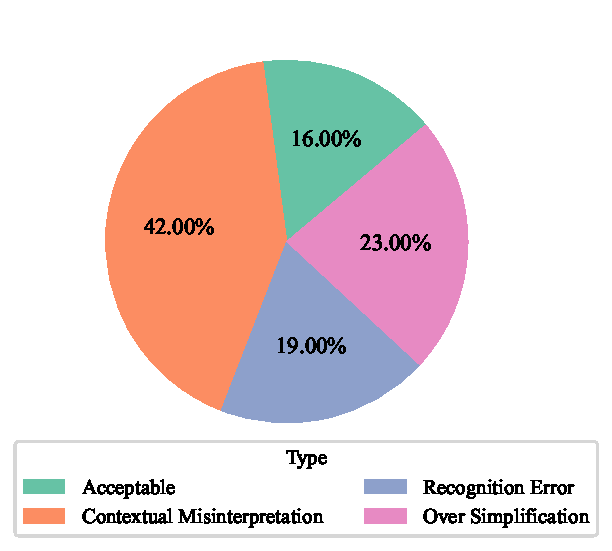
\includegraphics[width=0.8\linewidth]{figs/pie_chart.pdf}
    \caption{Manual analysis of the generated captions. }
    \label{fig:error_pie_chart}
\end{figure}


\begin{figure*}
    \centering
    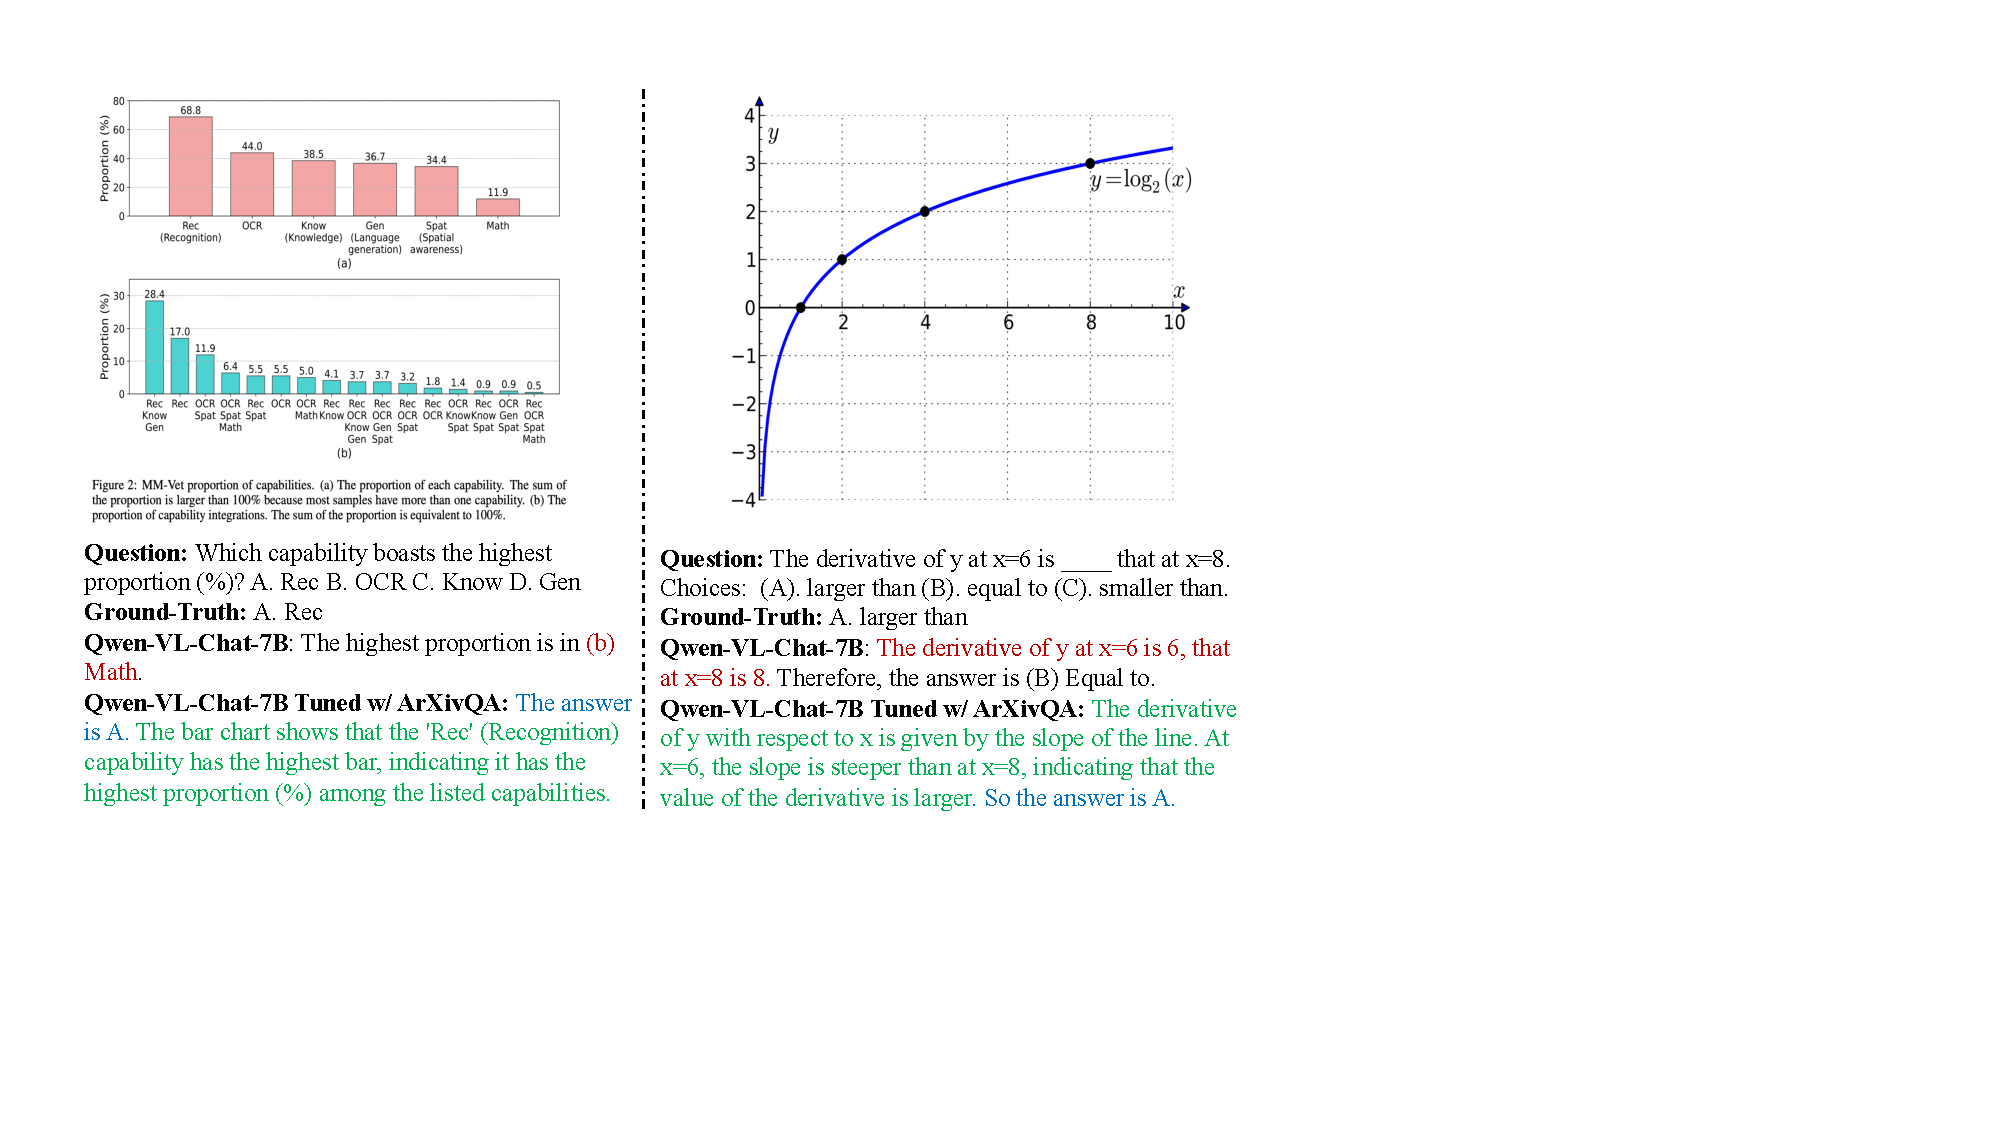
\includegraphics[width=0.62\linewidth]{figs/mathvista_case_study_v2.pdf}
    \caption{ArXivQA enables the model not only to answer questions related to scientific figures in papers (left) but also to improve mathematical understanding ability (right). The model not only selects correct options but also gives reasonable rationale.}
    \label{fig:math_case_study}
\end{figure*}

\paragraph{Manual Evaluation of Generated Captions} 
\label{subsubsec:manual_eval}
We conduct a manual inspection for single-figure captioning results. To ensure a more informed evaluation, we focus on a paper from the CS domain, leveraging our domain knowledge to assess caption quality better. 
The quality of generated captions is assessed by scrutinizing the figure, the ground-truth caption, the paper title, and the abstract.
We categorize captions into the following quality types according to our preliminary inspection: (1) \emph{Acceptable}, where captions accurately encapsulate the scientific figure's essence, aligning with the intended information of the ground-truth; (2) \emph{Over Simplification}, instances where the model oversimplifies content, offering a broad overview while neglecting specific details and nuances present in the ground truth; (3) \emph{Recognition Error}, where the model inaccurately recognizes and describes key visual and textual elements in the scientific figure, such as colors, numerical values, or textual context; and (4) \emph{Contextual Misinterpretation}, where the model misinterprets the specific context of the scientific figure, resulting in captions relevant in a generic sense but inaccurate for the given figure. Visualized generated captions of different types are shown in Figure~\ref{fig:caption_type} of Appendix~\ref{apx:caption_type}.
The results of 100 manually examined captions are depicted in Figure~\ref{fig:error_pie_chart}, revealing that only 16\% of captions are deemed acceptable when compared to human-written ones. 
Among unsatisfactory captions, contextual misinterpretation emerges as the dominant issue, suggesting a need for incorporating more contextual information as suggested in Table~\ref{tab:cap_with_meta_ret}. Oversimplification is another concern, with generic captions identified. Additionally, 23\% and 19\% of examined captions suffer from the oversimplification issue and recognition errors in reported numbers/texts in the caption, respectively. The former is attributed to the highly frequent simple caption in the training dataset and the latter issue could be addressed through potential integration with OCR results.
% In summary,  underscores opportunities to enhance captioning quality. 
Our manual evaluation suggests future efforts may benefit from incorporating additional context clues, such as paper metadata, improving the model's fundamental perception abilities, and utilizing external information.


% The error distribution comes from Figure~\ref{fig:error_pie_chart} shows that 16\% of the captions are perceived as acceptable compared with the human-written ones, indicating sufficient room for further improvements.
% Among the unsatisfactory captions, the most dominant type is contextual misinterpretation, which could be alleviated by incorporating more contextual information.
% Another issue is oversimplification, where the captions are generic to the present figure, such as (a) in Figure X.
% Also, 19\% of examined captions suffer from the recognition ability of the base model, i.e., the numbers are wrongly reported, which we think can be combined with OCR results.
% In summary, our manual evaluation suggests that future endeavors can be conducted to improve the captioning quality by incorporating more context clues, such as meta data of the paper, and improve the fundamental perception ability of the model.
% Acceptable 0.16
% Over Simplification 0.23
% Contextual Misinterpretation 0.42
% Recognition Error 0.19


\paragraph{Case Study of MathVista}
We conduct case studies to illuminate the tuning effects facilitated by our ArXivQA dataset. In the left segment of Figure~\ref{fig:math_case_study}, ArXivQA helps the model accurately answer a question related to the presented bar plot. 
% Notably, our ArXivQA, rooted in figures extracted from scientific papers, extends its impact beyond visual data. 
The right part in Figure~\ref{fig:math_case_study} demonstrates that ArXivQA can enhance algebraic reasoning abilities. Here, a question involving the derivative of a function is correctly answered, accompanied by a lucid reasoning rationale.
Figure~\ref{fig:geometry_fail} in Appendix~\ref{apx:failure_mathvista} highlights a challenging geometry problem where both models generate hallucinated outputs. 
These illustrative cases collectively affirm the efficacy of our dataset.
% reinforcing the observed quantitative accuracy improvements. 
% These nuanced examinations not only provide a qualitative understanding of the tuning effects but also underscore the dataset's broader impact on diverse mathematical reasoning tasks.


% We further present case studies to understand the improvement of the tuning effect of our ArXivQA dataset. As shown in the left part of Figure~\ref{fig:math_case_study}, the model after fine-tuning produces a correct answer for the question related to the presented bar plot. While our ArXivQA is constructed based on the figures extracted from scientific papers, the right case in Figure~\ref{fig:math_case_study} suggests that fine-tuning may also improve the algebraic reasoning ability, where a question of function derivative is correctly answered with reasoning rationale.
% We also present a failed geometry problem in Figure~\ref{fig:geometry_fail} in the Appendix where we found both models produce hallucinated outputs for a challenging geometry problem. Overall, these intuitive cases confirm the effectiveness of our dataset, echoing previous quantitative accuracy boost.

\section{Conclusion}
\label{sec:conclusion}
Our work introduces Multimodal ArXiv, comprising ArXivCap and ArXivQA, aims at advancing the scientific comprehension of LVLMs. 
Experiments show that fine-tuning on ArXivQA notably enhances LVLMs' mathematical reasoning capabilities. 
Moreover, our comprehensive evaluations across four vision-to-text tasks on ArXivCap underscore the challenges in understanding scientific figures for LVLMs, while highlighting the substantial improvements achieved by in-domain training. Our error analysis offers valuable insights for the ongoing development of LVLMs.
% , paving the way for future advancements in multimodal understanding within scientific domains.

% In this paper, we introduce Multimodal ArXiv, consisting of ArXivCap and ArXivQA for benchmarking and improving the scientific understanding of LVLMs. 
% We find that fine-tuning on ArXivQA significantly boosts the mathematical reasoning ability of LVLMs.
% Extensive evaluation results of four vision-to-text tasks on ArXivCap reveal the limited comprehension of LVLMs for scientific figures, and that in-domain training yields substantial improvements.
% Our error analysis provides insights for future development of LVLMs.

% Additionally, we leverage GPT-4V to generate a question-answering dataset using caption-figure pairs, which has proven effective in enhancing the mathematical reasoning abilities of LVLMs.
% By providing this dataset, we anticipate fostering a rich avenue for further studies, ultimately advancing LVLMs.



\section*{Limitations}
Our study has several limitations worth noting. Firstly, our exploration may not encompass the full spectrum of LVLMs due to the rapid evolution of architectures and training methodologies such as parameter-efficient tuning~\citep{hu2021lora,ma2024paramtuning}.
Nevertheless, we believe our dataset could still be effective for other LVLMs and the findings are generalizable.
We show that our ArXivQA dataset could also boost LLaVA-series models across scientific understanding benchmarks in Appendix~\ref{apx:llava}.
Secondly, our Multimodal ArXiv dataset sources from ArXiv papers due to their accessibility and open-source licenses. This approach may overlook the diversity of disciplines and data modalities present in the broader scientific literature. 
Future research could incorporate a broader range of datasets and domains to enrich the coverage of scientific knowledge, and explore dynamic data selection methods to improve performance and sample efficiency~\citep{li-etal-2021-dynamic,chen2024vlm_select}.

% Future research could incorporate a broader range of datasets and domains to enrich the coverage of scientific knowledge, and explore dynamic data selection methods for better performance and sample efficiency~\citep{li-etal-2021-dynamic,chen2024vlm_select}.



% Bibliography entries for the entire Anthology, followed by custom entries
%\bibliography{anthology,custom}
% Custom bibliography entries only
\section*{Acknowledgments}

We thank Albert Gu for helpful discussion regarding the model architecture, and
more importantly for sending us daily hippo videos.
We thank Together Computer
for providing portions of the compute used to train models in this paper.
We gratefully acknowledge the support of NIH under No. U54EB020405 (Mobilize), NSF under Nos. CCF1763315 (Beyond Sparsity), CCF1563078 (Volume to Velocity), and 1937301 (RTML); ARL under No. W911NF-21-2-0251 (Interactive Human-AI Teaming); ONR under No. N000141712266 (Unifying Weak Supervision); ONR N00014-20-1-2480: Understanding and Applying Non-Euclidean Geometry in Machine Learning; N000142012275 (NEPTUNE); NXP, Xilinx, LETI-CEA, Intel, IBM, Microsoft, NEC, Toshiba, TSMC, ARM, Hitachi, BASF, Accenture, Ericsson, Qualcomm, Analog Devices, Google Cloud, Salesforce, Total, the HAI-GCP Cloud Credits for Research program,  the Stanford Data Science Initiative (SDSI),
Department of Defense (DoD) through the National Defense Science and
Engineering Graduate Fellowship (NDSEG) Program, 
Wu Tsai Neuroscience Stanford Interdisciplinary Graduate Fellowship,
and members of the Stanford DAWN project: Facebook, Google, and VMWare. The U.S. Government is authorized to reproduce and distribute reprints for Governmental purposes notwithstanding any copyright notation thereon. Any opinions, findings, and conclusions or recommendations expressed in this material are those of the authors and do not necessarily reflect the views, policies, or endorsements, either expressed or implied, of DARPA, NIH, ONR, or the U.S. Government.
Atri Rudra’s research is supported by NSF grant CCF-1763481.

\bibliography{11_references}
\appendix

\section{Details of Multimodal ArXiv}
\label{apx:arxiv_cap}


\subsection{Caption Cleaning}
\label{apx:caption_clean}

We apply a Python tool to clean the original caption and Table~\ref{tab:pylatexenc_clean} illustrates the caption before and after cleaning. 
\begin{table}[tbh!]
    \centering
    \begin{tabular}{p{3cm}  p{3cm}}
    \toprule
       Before Cleaning & After Cleaning \\
       \midrule
       A 1995 Hale Telescope H$\alpha$ image of the Guitar Nebula (20 angstrom filter at 6564 angstroms). The cometary neck connecting to a spherical bubble are clearly evident. Credit: \textbackslash cite\{cha02\}. &
        A 1995 Hale Telescope H$\alpha$ image of the Guitar Nebula (20 angstrom filter at 6564 angstroms). The cometary neck connecting to a spherical bubble are clearly evident. Credit: \textless cit.\textgreater. \\ 
       \midrule
       As Fig. \textbackslash ref\{z0\} except at $z\sim 6$ ($z=4.37$ in the EdS model). &
    As Fig. \textless ref\textgreater~except at $z\sim 6$ ($z=4.37$ in the EdS model). \\ 
 
       \bottomrule
    \end{tabular}
    \caption{Caption before and after cleaning using pylatexenc.}
    \label{tab:pylatexenc_clean}
\end{table}


\subsection{Illustration Cases of Multimodal ArXiv}
\label{apx:case_illustrations}
We provide illustrated cases from our dataset for a better understanding.
Figure~\ref{fig:single_figure_pair} demonstrates a typical single figure-caption pair, and Figure~\ref{fig:multi_figure_case} shows the multiple figure-caption case.
Figure~\ref{fig:qa_case_1}, \ref{fig:qa_case_2}, \ref{fig:qa_case_3} and \ref{fig:qa_case_4} illustrate the cases from our ArXivQA dataset, covering different figure types and containing diverse questions.



\begin{figure}[htb!]
    \centering
    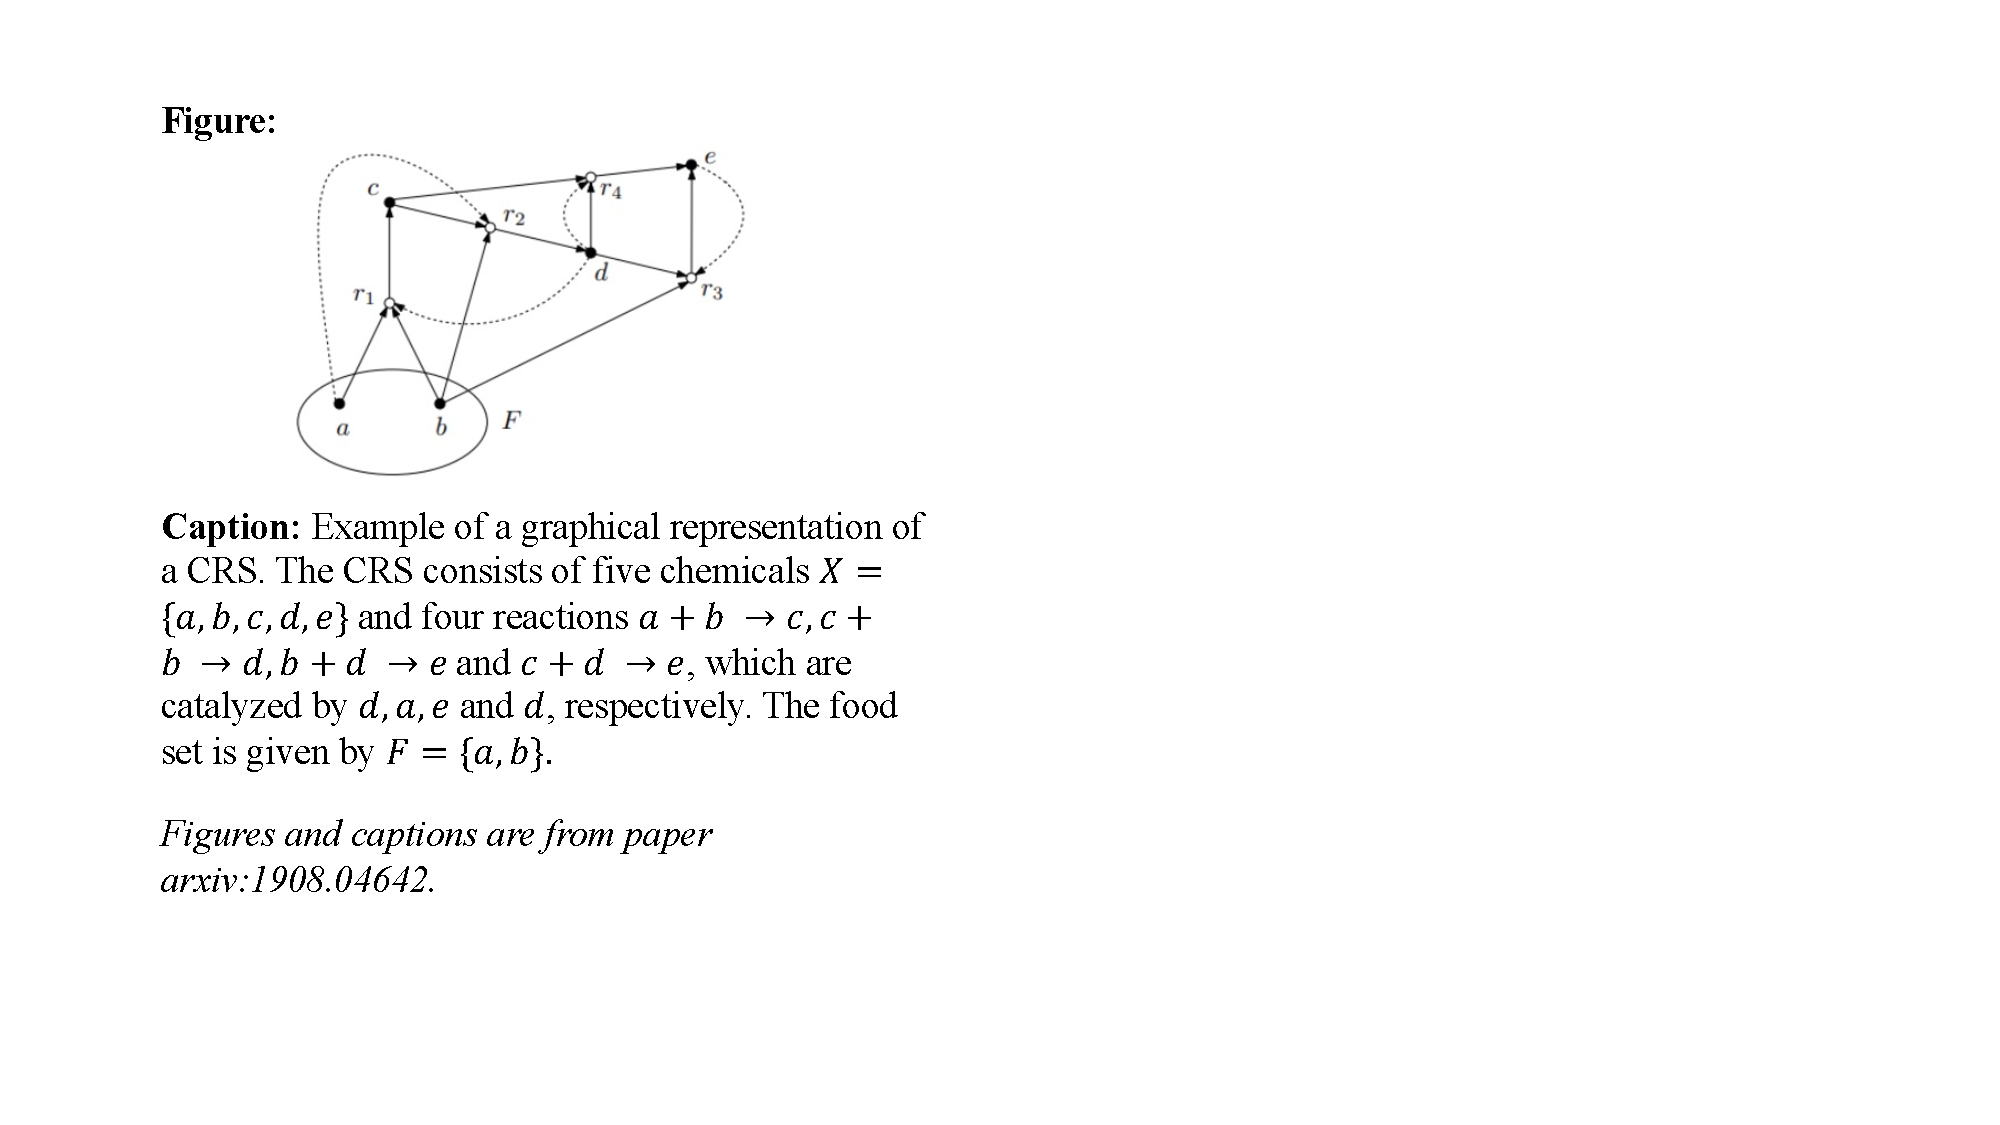
\includegraphics[width=\linewidth]{figs/single-figure-v2.pdf}
    \caption{A single-figure caption pair in our ArXivCap dataset.}
\label{fig:single_figure_pair}
\end{figure}


\begin{figure*}[t!]
    \centering
    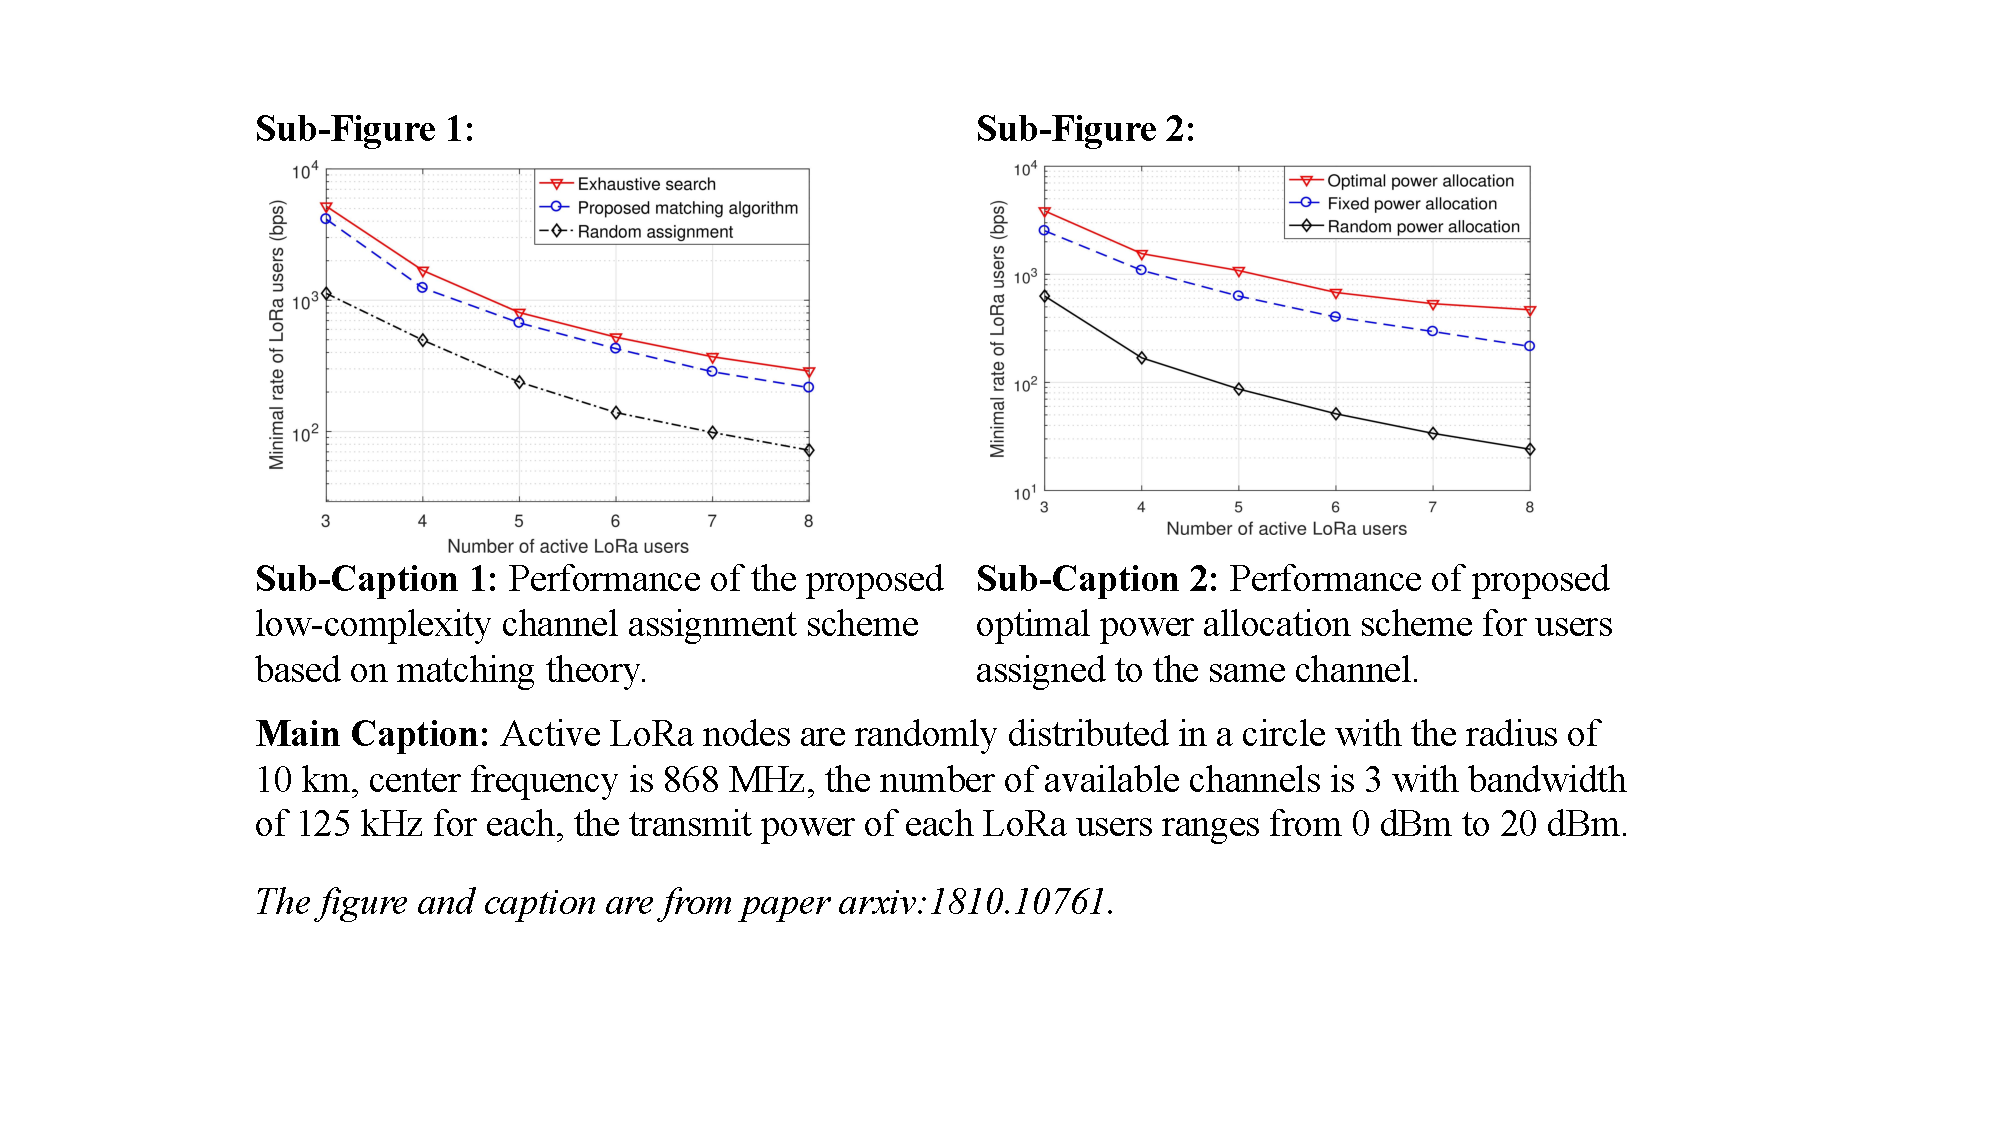
\includegraphics[width=0.85\linewidth]{figs/multiple-figure-v2.pdf}
    \caption{A multiple-figure caption pair in our ArXivCap dataset.}
    \label{fig:multi_figure_case}
\end{figure*}

\subsection{Caption Word Cloud}
\label{apx:caption_word_cloud}

We visualize the word cloud of captions in our ArXivCap dataset in Figure~\ref{fig:word_cloud}. It can be seen that the captions have a diverse vocabulary for describing the different figures in the academic papers.
\begin{figure}[t!]
    \centering
    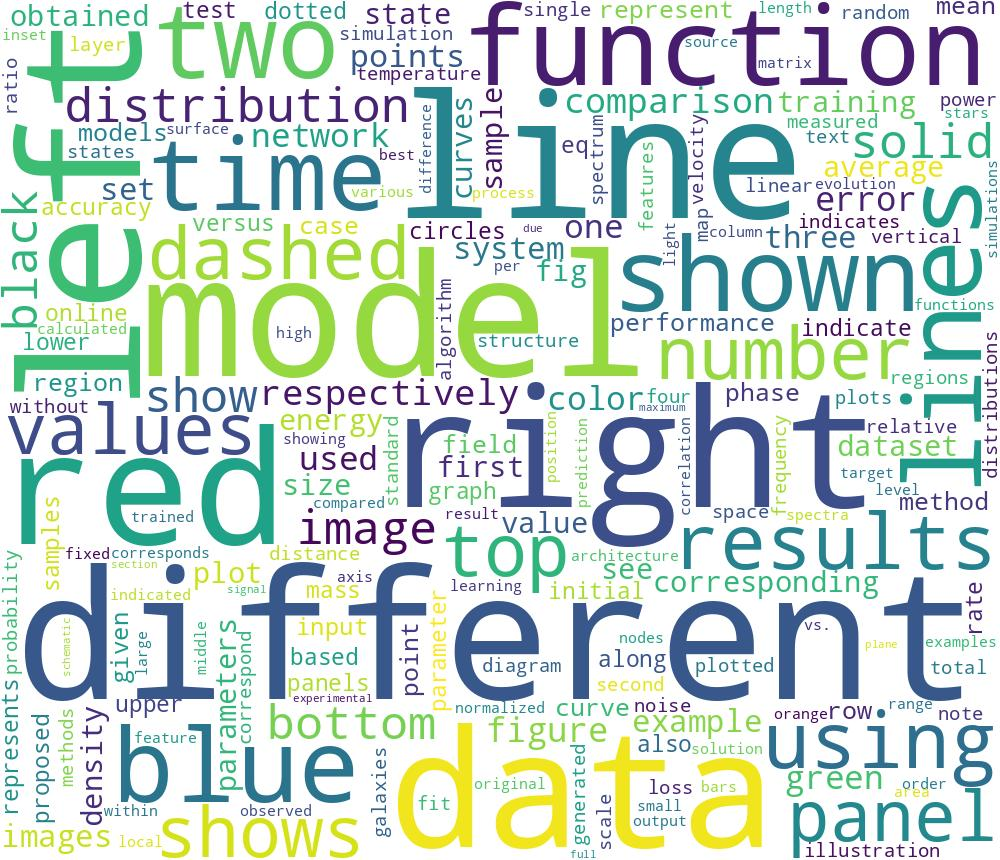
\includegraphics[width=\linewidth]{figs/word_cloud.jpg}
    \caption{Word cloud visualization of captions in our ArXivCap dataset.}
    \label{fig:word_cloud}
\end{figure}




\begin{figure*}[tbh!]
    \centering
    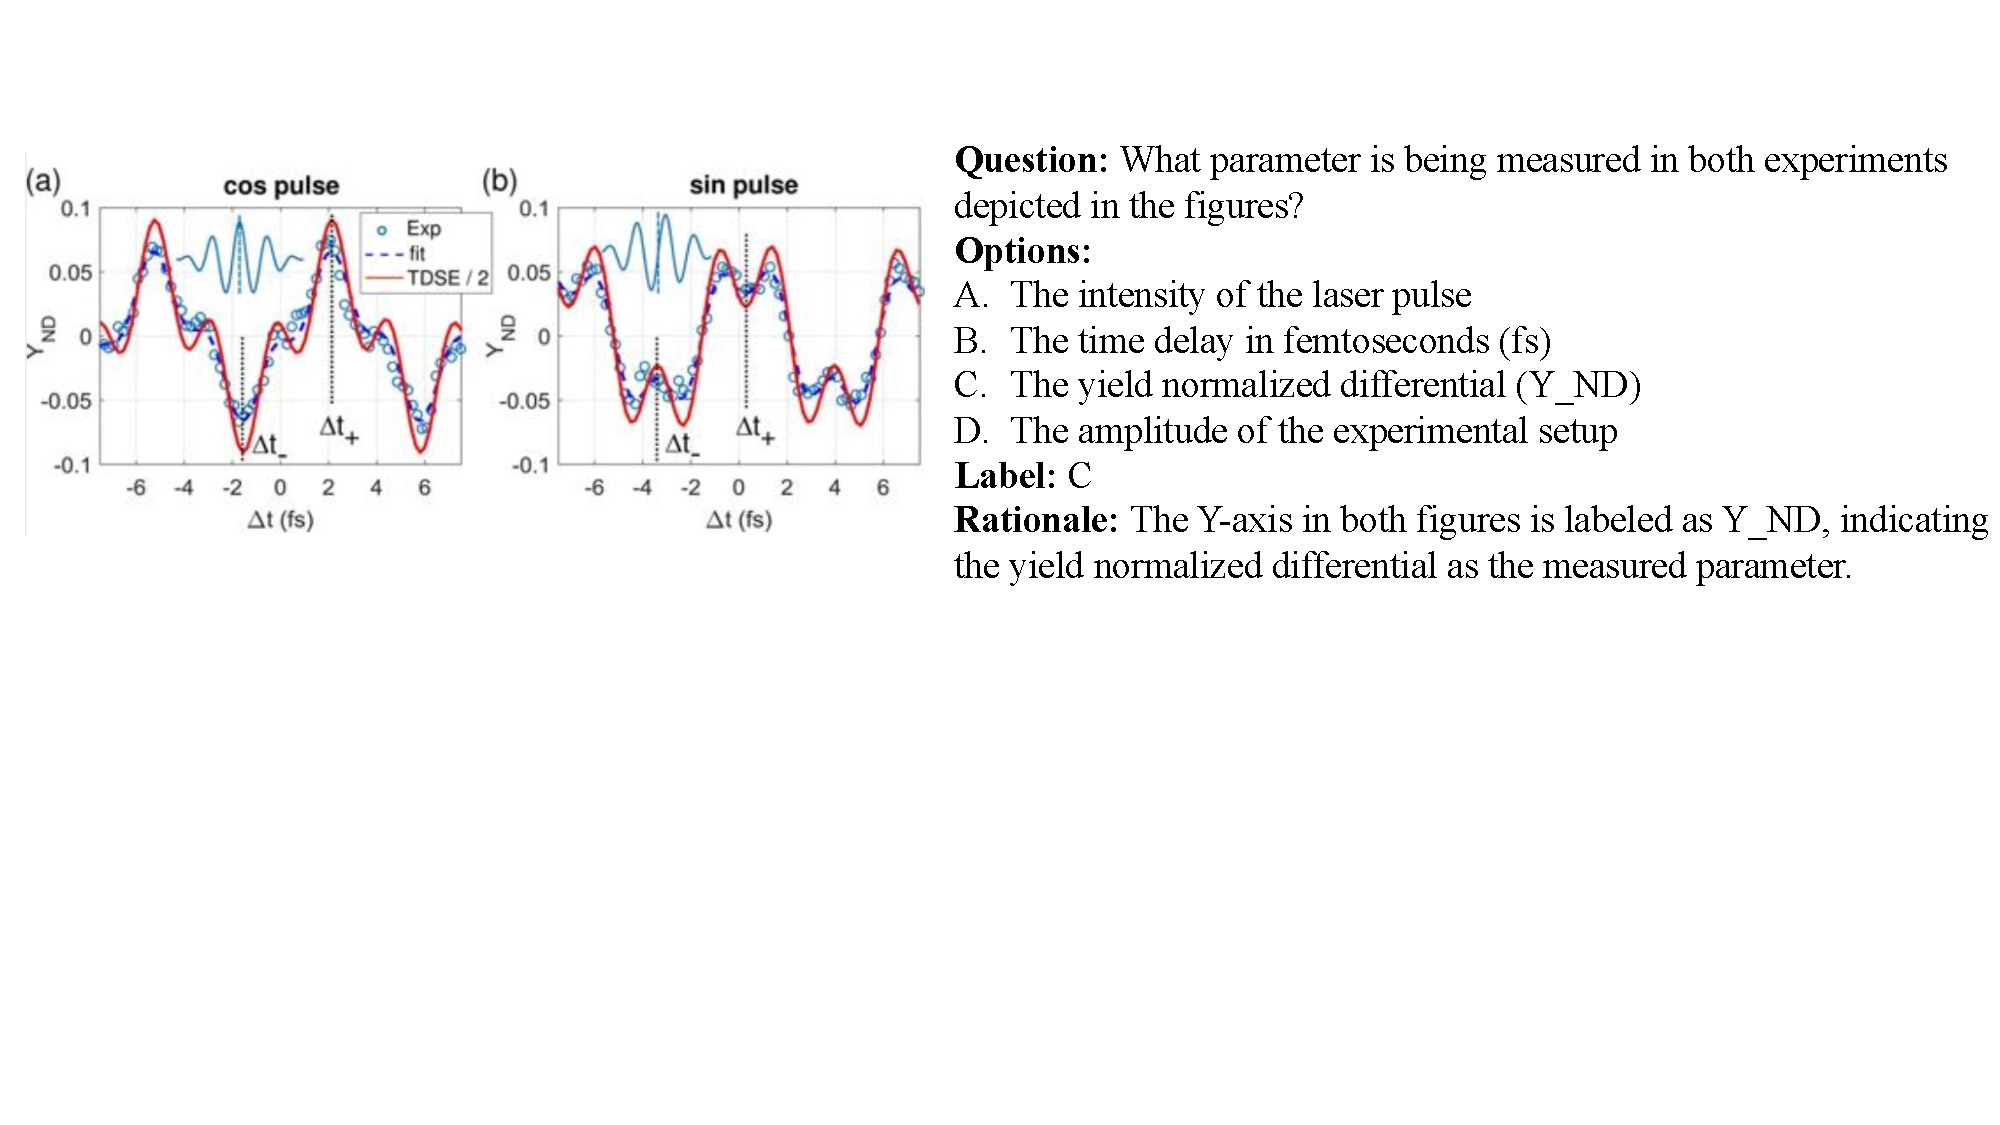
\includegraphics[width=0.85\linewidth]{figs/arxivqa_case1.pdf}
    \caption{A case from our ArXivQA dataset.}
    \label{fig:qa_case_1}
\end{figure*}



\begin{figure*}[tbh!]
    \centering
    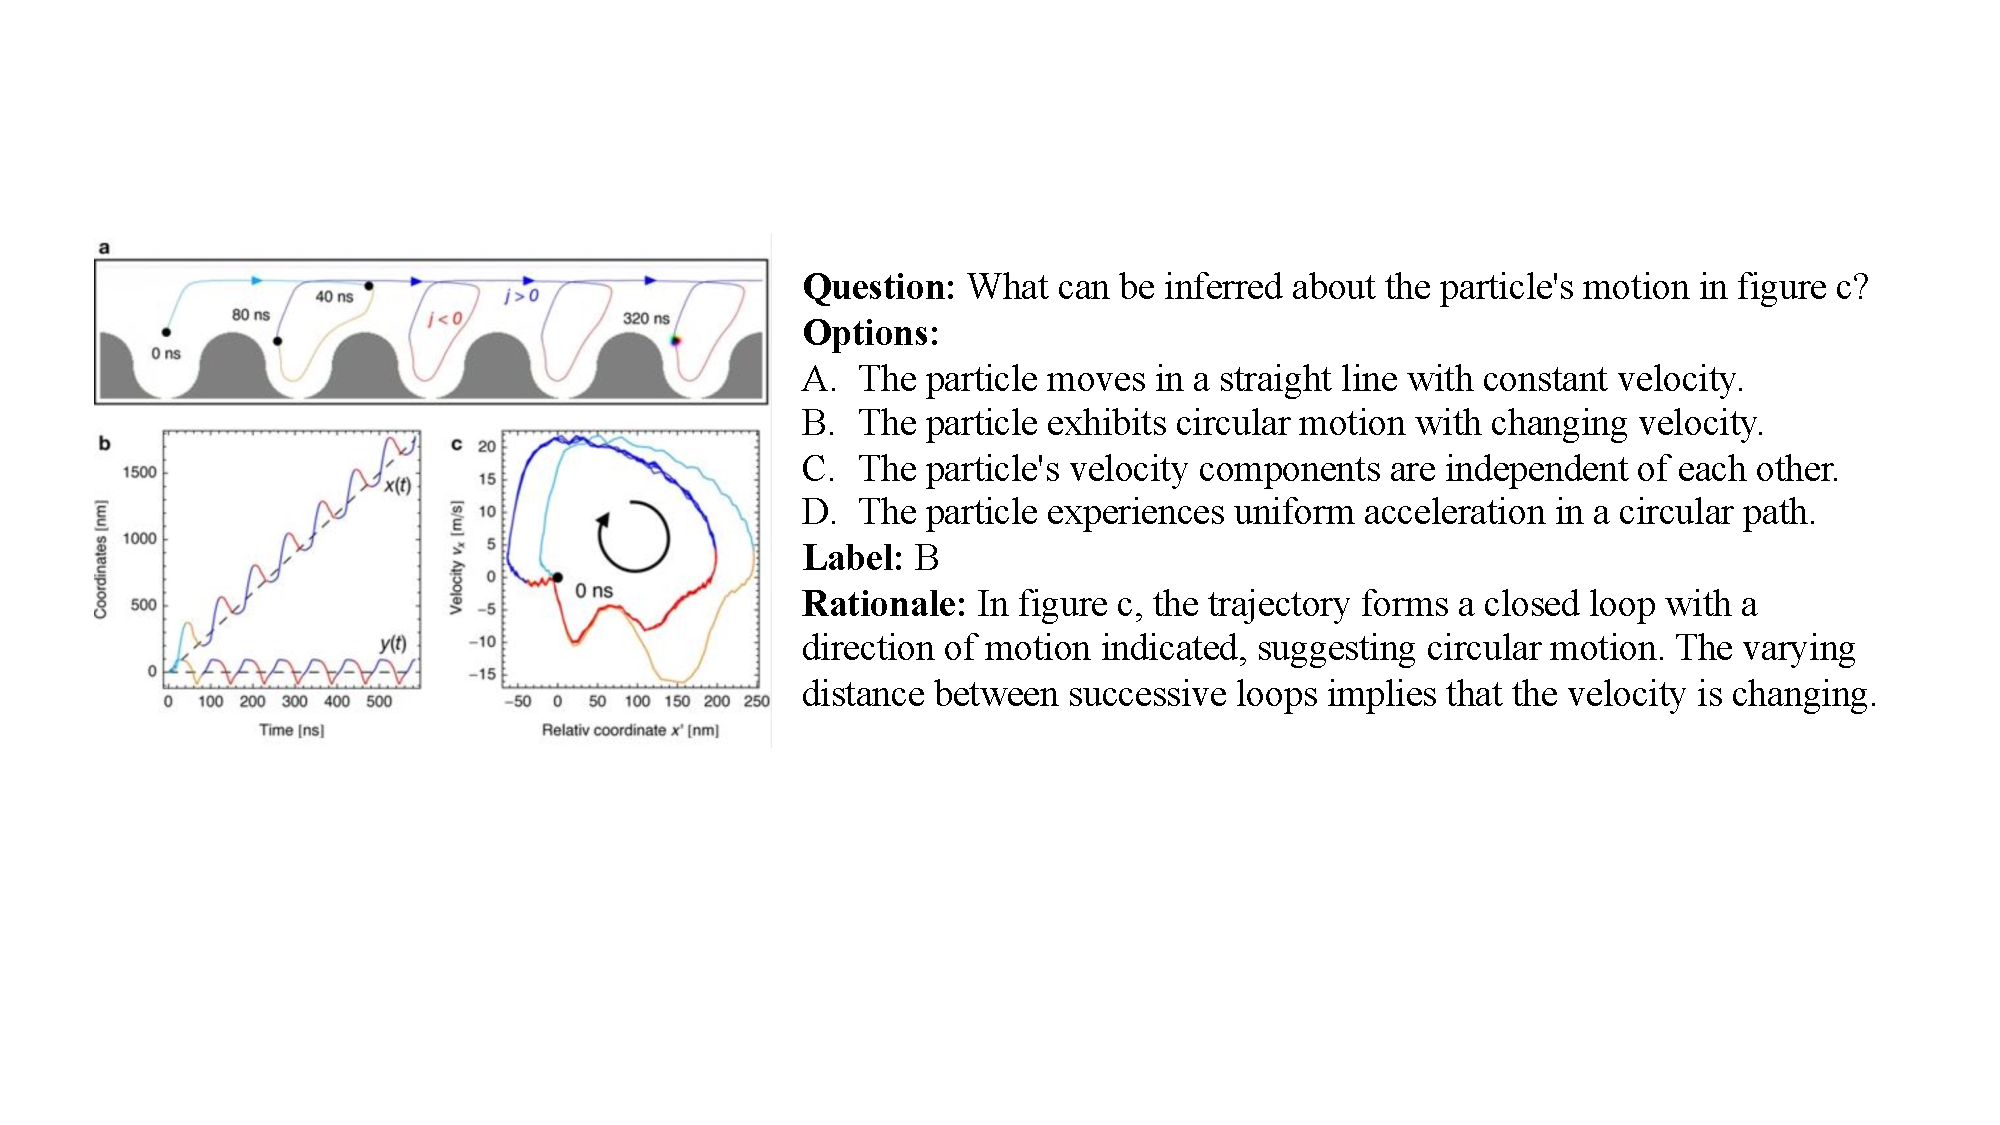
\includegraphics[width=0.85\linewidth]{figs/arxivqa_case2.pdf}
    \caption{A case from our ArXivQA dataset.}
    \label{fig:qa_case_2}
\end{figure*}



\begin{figure*}[tbh!]
    \centering
    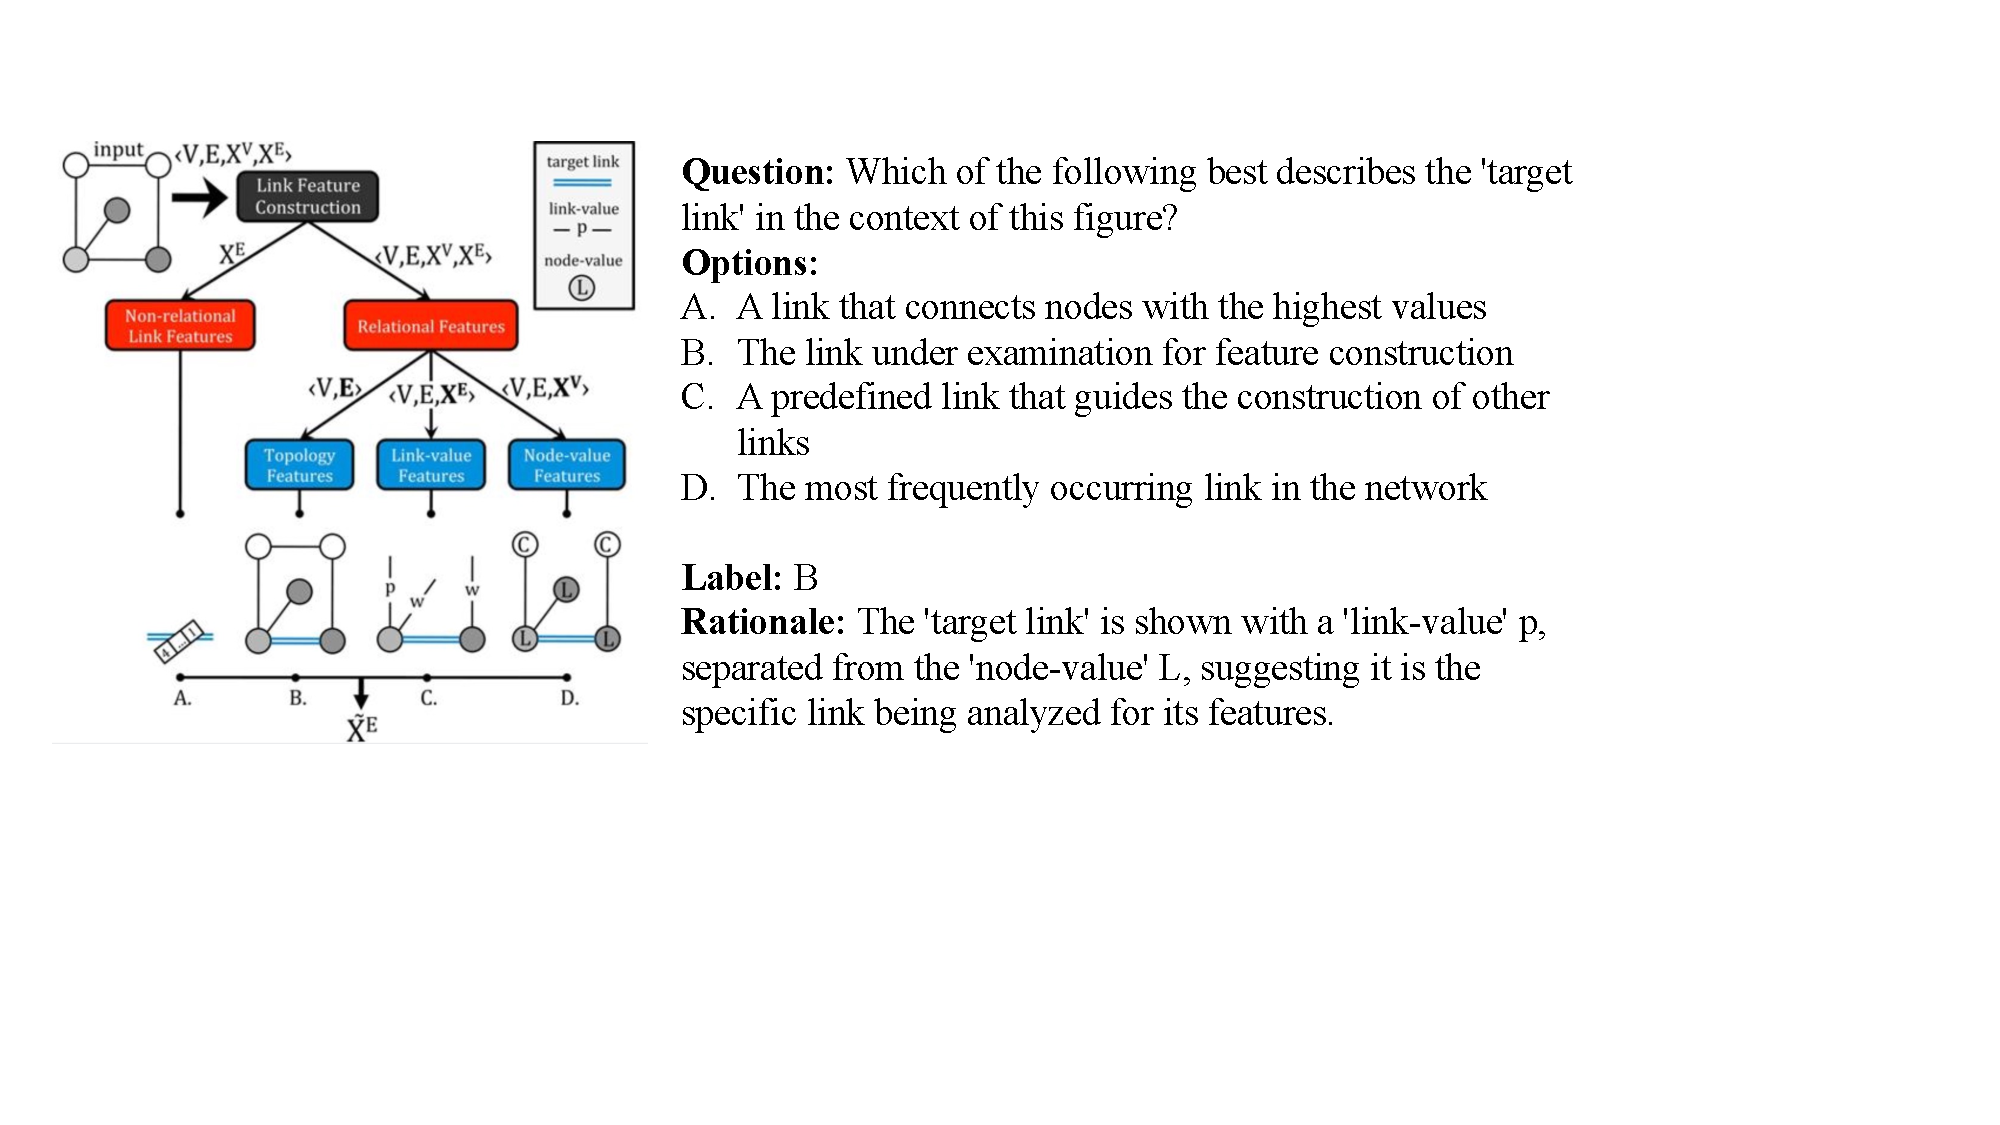
\includegraphics[width=0.85\linewidth]{figs/arxivqa_case3.pdf}
    \caption{A case from our ArXivQA dataset.}
    \label{fig:qa_case_3}
\end{figure*}



\begin{figure*}[tbh!]
    \centering
    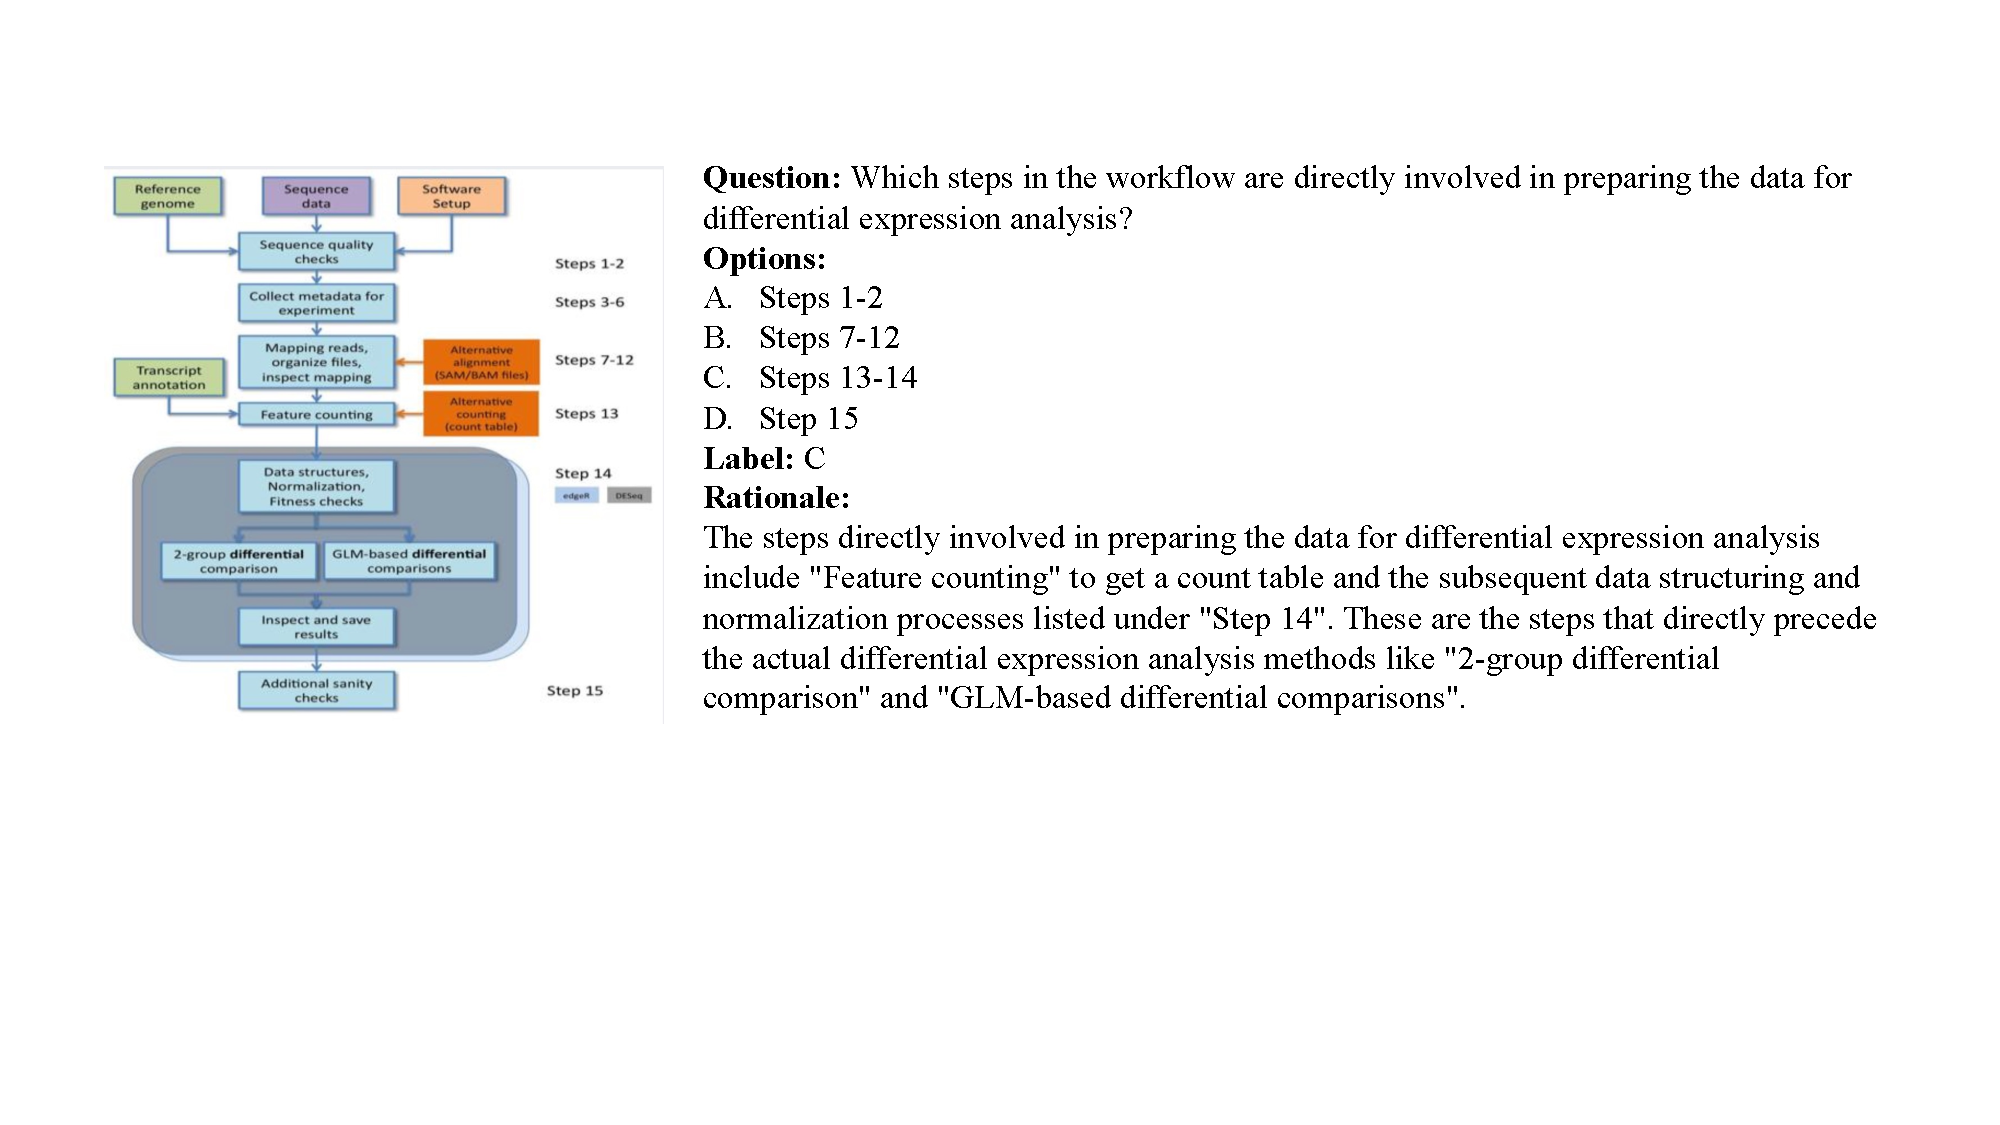
\includegraphics[width=0.85\linewidth]{figs/arxivqa_case4.pdf}
    \caption{A case from our ArXivQA dataset.}
    \label{fig:qa_case_4}
\end{figure*}
\begin{table}[tbh!]
    \centering
    \small 
    \resizebox{\linewidth}{!}{
    \begin{tabular}{l|c}
    \toprule
       Domain  & Full Name \\
       \midrule     
        dg-ga & Differential Geometry \\
        acc-phys & Accelerator Physics  \\
        solv-int & Exactly Solvable and Integrable Systems  \\
        q-alg &  Quantum Algebra and Topology \\
        atom-ph &  Atomic, Molecular and Optical Physics \\
        alg-geom & Algebraic Geometry  \\
        comp-gas &  Cellular Automata and Lattice Gases \\
        supr-con & Superconductivity  \\
        chem-ph &  Chemical Physics \\
        mtrl-th & Materials Theory  \\
        adap-org &  Adaptation, Noise, and Self-Organizing Systems \\
        patt-sol & Pattern Formation and Solitons  \\
        chao-dyn &  Chaotic Dynamics \\
        cmp-lg &  Computation and Language \\
        econ & Economics  \\
        hep-lat & High Energy Physics - Lattice  \\
        nucl-ex & Nuclear Experiment  \\
        q-fin &  Quantitative Finance \\
        math-ph &  Mathematical Physics \\
        nucl-th &  Nuclear Theory \\
        gr-qc & General Relativity and Quantum Cosmology  \\
        hep-ex & High Energy Physics - Experiment  \\
        hep-th & High Energy Physics - Theory \\
        nlin & Nonlinear Sciences \\
        hep-ph & High Energy Physics - Phenomenology \\
        q-bio & Quantitative Biology \\
        quant-ph & Quantum Physics \\
        eess & Electrical Engineering and Systems Science \\
        stat & Statistics \\
        astro-ph & Astrophysics \\
        physics & Physics  \\
        cond-mat & Condensed Matter \\
        math & Mathematics \\
        cs & Computer Science \\
       \bottomrule
    \end{tabular}}
    \caption{Name of each domain.}
    \label{tab:domain-full-name}
\end{table}



\begin{table}[t!]
    \centering
    \tiny 
    \begin{tcolorbox}
Multiple-choice Question Answer Pairs Generation for Scientific Figures

\textbf{Guideline}

The goal of this task is to create answerable multiple-choice questions based on figures from scientific papers, to improve the ability of a large vision language model.

The questions should be challenging, and require college-level reasoning. The type of questions should be diverse. The question should be answerable based on the figure. The answer should be one of the answer choices. The answer choices should be plausible and challenging. 


\textbf{Format}

Below is an example of the format of the input and output for the task.

\textbf{Input}

Figures: [Figures input in the task]

\textbf{Output}

Question: [Question]

Answer Options: [Answer choices, a bullet list.]

Correct Choice: [Correct answer choice, e.g., A]

Rationale: [Rationale for the correct answer, explain why the answer is correct]
    \end{tcolorbox}
    \caption{Prompt used for GPT-4V to generate QA pairs based on scientific figures.}
    \label{tab:prompt_for_ArXivqa}
\end{table}
\subsection{ArXivQA Prompting Template}
\label{apx:prompt_template}
The prompt used to query GPT-4V is provided in Table~\ref{tab:prompt_for_ArXivqa}.

\subsection{Quality Analysis of ArXivQA}
\begin{table*}[t!]
    \centering
    \tiny  
    \begin{tcolorbox}
1. Ensuring Factual Integrity and Clear Presentation:\\
- Factual Alignment: Ensure questions and options are grounded in accurate reflections of the chart data.\\
- Visual Clarity: Maintain high-resolution charts to ensure that all pertinent details are discernible.\\
- Unambiguous Textual Information: Employ precise and unambiguous language to formulate questions and answers, thereby mitigating potential misinterpretations.\\
2. Ensuring Relevance and Integrated Comprehensiveness:\\
- Question and Option Relevance: Charts must align with their questions, and all options should be applicable and relevant to the given data.\\
- Comprehensive Integration: Guarantee the provision of comprehensive information necessary for the interpretation of the chart and the resolution of the question, ensuring a cohesive amalgamation of textual and visual data.\\ 
3. Promoting Fairness and Avoiding Bias:\\
- Equitable Content: Strive for impartiality in the dataset to prevent bias and ensure fair representation of diverse groups and perspectives.\\

Grading Protocol:\\
Each criterion is to be rigorously evaluated for each dataset entry. The assessment is to be conducted on a qualitative scale with three distinct levels: High, Medium, and Low. These levels will denote the degree of conformity to the respective criterion:\\
- 1: High: The dataset entry exhibits exemplary adherence to the evaluation criterion, demonstrating a robust and comprehensive alignment with the specified standard.\\
- 0.5: Medium: The dataset entry meets the evaluation criterion to a moderate extent, indicating a satisfactory but not optimal congruence with the standard.\\
- 0 Low: The dataset entry falls short of the evaluation criterion, signaling a need for significant improvements to meet the standard.
    \end{tcolorbox}
    \caption{Annotator guideline of ArXivQA manual quality examination.}
    \label{tab:quality_analysis_ArXivqa}
\end{table*}

\begin{table}[t!]
    \centering
    \small 
    \begin{tabular}{@{}lc@{}}
         \toprule
         Aspect & Avg Score \\
         \midrule
        Factual Alignment & 0.6975 \\
        Visual Clarity & 0.9925 \\
        Unambiguous Textual Information & 0.9825 \\
        Question and Option Relevance & 0.9375 \\
        Comprehensive Integration & 0.905 \\
        Equitable Content & 1.0 \\
        \midrule
        Score Sum & 5.515 \\
        \bottomrule
    \end{tabular}
    \caption{Manual quality analysis of ArXivQA. The average scores for each aspect are presented.}
    \label{tab:quality_analysis_ArXivqa_result}
\end{table}
To evaluate the quality of ArXivQA, we manually assess it from six different aspects. We develop a quality examination guideline for annotators, as shown in Table~\ref{tab:quality_analysis_ArXivqa}, which addresses various aspects of the QA pairs.
We sample 100 examples and ask four authors to conduct the quality analysis. The four authors are divided into two groups, with each group tasks with evaluating 50 examples across six sub-aspects, according to the grading protocol. 

The evaluation results are presented in Table~\ref{tab:quality_analysis_ArXivqa_result}.
We find that most samples feature clear, high-quality images with clear and high-quality images, with unambiguous question and option descriptions. However, a small fraction of the generated questions may be unanswerable due to mis-recognizing elements in the figures, as reflected by lower factual alignment scores. Additionally, we consider samples with an aggregate score of 5 or higher from both annotators to be of sufficient quality. Under this stringent criterion, 79 out of 100 samples meet the threshold, demonstrating that the dataset's quality is generally satisfactory.

\section{Evaluation Details}
\label{apx:evaluation_details}
\subsection{Details of Evaluated Models}


\paragraph{BLIP2}~\citep{li2023blip2}, 
introduces a lightweight Q-Former designed to bridge modality gaps and leverages frozen LLMs. Leveraging LLMs, BLIP-2 can conduct zero-shot image-to-text generation using natural language prompts. We select the \texttt{BLIP2-OPT-6.7B} version for evaluation.\footnote{\url{https://huggingface.co/Salesforce/blip2-opt-6.7b}}


\paragraph{InstructBLIP}~\citep{dai2023instructblip} employs an instruction-aware visual feature extraction module based on BLIP2~\citep{li2023blip2} and is trained with unified multimodal instruction tuning datasets. We choose \texttt{InstructBLIP-Vicuna-7B} for evaluation.\footnote{\url{https://huggingface.co/Salesforce/instructblip-vicuna-7b}}.



\paragraph{LLaVA}~\citep{liu2023llava},
adopts Vicuna models as the backbone LLM and is trained on the ChatGPT/GPT-4 generated instruction tuning dataset.
LLaVA-v1.5~\citep{liu2023llava15} improves on LLaVA models by employing curated task datasets and an enhanced modality alignment module.
We evaluate both \texttt{LLaVA-v1.5-7B}\footnote{\url{https://huggingface.co/liuhaotian/llava-v1.5-7b}} and \texttt{LLaVA-v1.5-13B}.\footnote{\url{https://huggingface.co/liuhaotian/llava-v1.5-13b}}


\paragraph{Flamingo}~\citep{Alayrac2022FlamingoAV} pioneers the development of LVLMs by introducing a cross-gated layer for LLMs to produce visual-grounded text. The training dataset
consists of interleaved visual data and text from the web pages, enabling it to generate free-form text as the output. We select the open-source implementation \texttt{OpenFlamingo-9B}~\citep{awadalla2023openflamingo} for evaluation.\footnote{\url{https://huggingface.co/openflamingo/OpenFlamingo-9B-vitl-mpt7b}}

\begin{table*}[t!]
    \centering
\tiny 
\begin{tcolorbox}
Annotation Instruction:\\
As an annotator, your role is to serve as an unbiased and objective judge in evaluating the accuracy of captions produced by a Large Vision-Language Model (LVLM) for scientific figures. These figures are extracted from academic papers, and to aid your assessment, we will provide you with the paper's title and abstract for necessary context.

You will be presented with the original caption—referred to as the 'ground truth'—and the LVLM generated caption, termed the 'prediction'. You could take into account the context given by the paper's title and abstract for background knowledge, comparing it critically with both captions.

In your assessment, please pay attention to the factual alignment, including but not limiting to the following aspects:\\
- Numerical data and statistics: Verify their accuracy and correspondence to the data presented in the figure.\\
- Symbols: Check for correct representation and usage in the context of the scientific subject matter.\\
- Factual content: Ensure all facts are consistent with those stated in the ground truth caption and the paper's content.\\

<title>{title}</title>\\
<abstract>{abstract}</abstract>\\
<ground truth>{gt}</ground truth>\\
<prediction>{pred}</prediction>\\

Compare the prediction to the ground truth, provide a brief analysis, and assign a score using one of the following quality labels: <Perfect>, <Good>, <Fair>, <Poor>, <Incorrect>.

Below we describe the detail criteria for score:
<Perfect>: The prediction is almost identical to the ground truth, with only minor, inconsequential differences that do not change the meaning. All numerical data, symbols, and factual content are accurate and consistent.\\
<Good>: The prediction is largely similar to the ground truth but has some noticeable differences that may slightly change the meaning. However, the core information is still correct, and the numerical data, symbols, and factual content are mostly accurate and consistent with the figure content.\\
<Fair>: The prediction captures the basic idea of the ground truth but has significant differences that change the meaning in a way that cannot be ignored. There may be some inaccuracies or inconsistencies in the numerical data, symbols, or factual content when compared to the figure content.\\
<Poor>: The prediction is related to the ground truth but has serious errors or omissions that significantly change the meaning. The numerical data, symbols, or factual content may be largely inaccurate or inconsistent with the figure content.\\
<Incorrect>: The prediction is completely different or irrelevant to the ground truth, with no similarities between the two. The numerical data, symbols, and factual content are entirely inaccurate or inconsistent with the figure content.

Give a brief analysis within 100 words and then output a quality label wrapped with "<>".
    \end{tcolorbox}
    \caption{Prompt template designed for GPT-4 to evaluate generated captions based on the paper title, abstract, and ground truth.}
    \label{tab:prompt_for_gpt4_score_caption}
\end{table*}

\begin{table}[t!]
    \centering
    \small  
    \resizebox{\linewidth}{!}{
    \begin{tabular}{@{}lcccc@{}}
         \toprule
         Model & BLEU-2 & ROUGE-L & BERT-S & GPT-4 Score \\
         \midrule
BLIP-2-OPT-6.7B & 1.5 & 6.6 & 81.3 & 1.18 \\
InstructBLIP-Vicuna7B & 3.5 & 10.3 & 83.6 & 1.48 \\
LLaVA-1.5-7B & 2.3 & 10.4 & 83.3 & 1.80 \\
LLaVA-1.5-13B & 2.7 & 11.0 & 83.6 & 1.69 \\
OpenFlamingo-9B & 5.8 & 10.3 & 82.7 & 1.52 \\
IDEFICS-Instruct-9B & 2.1 & 9.3 & 83.8 & 1.55 \\
Qwen-VL-Chat & 4.7 & 11.1 & 82.0 & 1.81 \\
Qwen-VL-Chat tuned w/ ArXivCap & 8.6 & 15.3 & 83.2 & 2.03 \\
         \bottomrule
    \end{tabular}}
    \caption{Results of 500 single-figure captions generated by various models.}
    \label{tab:gpt4_score_single_caption}
\end{table}



\paragraph{IDEFICS} is another open-sourced implementation of Flamingo~\citep{Alayrac2022FlamingoAV}. Trained on publicly available image-text alignment pairs and instruction tuning datasets, it demonstrates comparable results with the original closed-source model on various image-text benchmarks. We select the \texttt{IDEFICS-Instruct-9B} for evaluation.\footnote{\url{https://huggingface.co/HuggingFaceM4/idefics-9b-instruct}}.

\paragraph{Qwen-VL-Chat}~\citep{Qwen-VL} is
a bilingual LVLM that supports both English and Chinese built on the Qwen LLM~\citep{qwen}. 
During the training phase, Qwen-VL-Chat adopts a packing strategy to create multiple images as inputs,
improving its ability to understand the vision context. We select the \texttt{Qwen-VL-Chat-7B} for evaluation.\footnote{\url{https://github.com/QwenLM/Qwen-VL}}



\paragraph{GPT-4V}
~\citep{gpt4v}, the proprietary vision-language models developed by OpenAI, which are shown to be powerful on various multi-modal tasks~\citep{yang2023dawn}. The API version we queried is \texttt{gpt-4-vision-preview}.

\paragraph{Bard}~\citep{bard}, a commercial LVLM developed by Google. We utilize the unofficial API\footnote{\url{https://github.com/dsdanielpark/Bard-API}} querying the model with our task prompts, accessed on \texttt{2023-11-17}.

\paragraph{Gemini 1.0 Pro Vision}~\citep{reid2024gemini}, a upgraded LVLM by Google. We utilize the official API querying the model with our task prompts, accessed on \texttt{2024-05-20}.


\subsection{Task Prompts}
We evaluate all the models with the same task prompts in our experiments, and the prompts for our four tasks are listed below:

\noindent\textbf{Single-Figure Captioning}:  \texttt{Create a caption for the provided figure.}

\noindent\textbf{Multiple-Figure Captioning} \texttt{Create a caption for the provided figures.}

\noindent\textbf{Contextualized Captioning}: We reuse the prompts in previous captioning tasks depending on the current figure type.

\noindent\textbf{Title Generation}: \texttt{
According to the figures and captions, generate a title for this paper. Title:} 


\subsection{GPT-4 Evaluation of Caption}
\label{apx:gpt4_eval}


In addition to BLEU-2, ROUGE-L, and BERT-S, we also utilize GPT-4 to evaluate a sample of 500 generated captions. Specifically, we employ GPT-4 for the evaluation of single-figure caption tasks following FairEval~\citep{wang2023large}.
The template for prompting GPT-4 to evaluate generated captions is presented in Table~\ref{tab:prompt_for_gpt4_score_caption}. GPT-4 is asked to perform an analysis and then produces a quality score, which is subsequently mapped to a scale from 1 to 5.
The results are presented in Table~\ref{tab:gpt4_score_single_caption}. We observe that the ROUGE-L metric exhibits the highest correlation with the GPT-4 Score (Pearson r = 0.91), followed by BLEU-2 (Pearson r = 0.64). BERT-S instead demonstrates a moderate correlation (Pearson r = 0.39).
The uniformly low GPT-4 scores across all models suggest that they struggle to produce satisfactory captions, which is consistent with the findings in our main paper. Notably, training on ArXivCap results in a significant 12\% improvement in the GPT-4 score compared to the original Qwen-VL-Chat model, leading to the most favorable outcomes in this evaluation.

\section{Error Analysis}
\label{apx:case}
\begin{figure*}[t!]
    \centering
    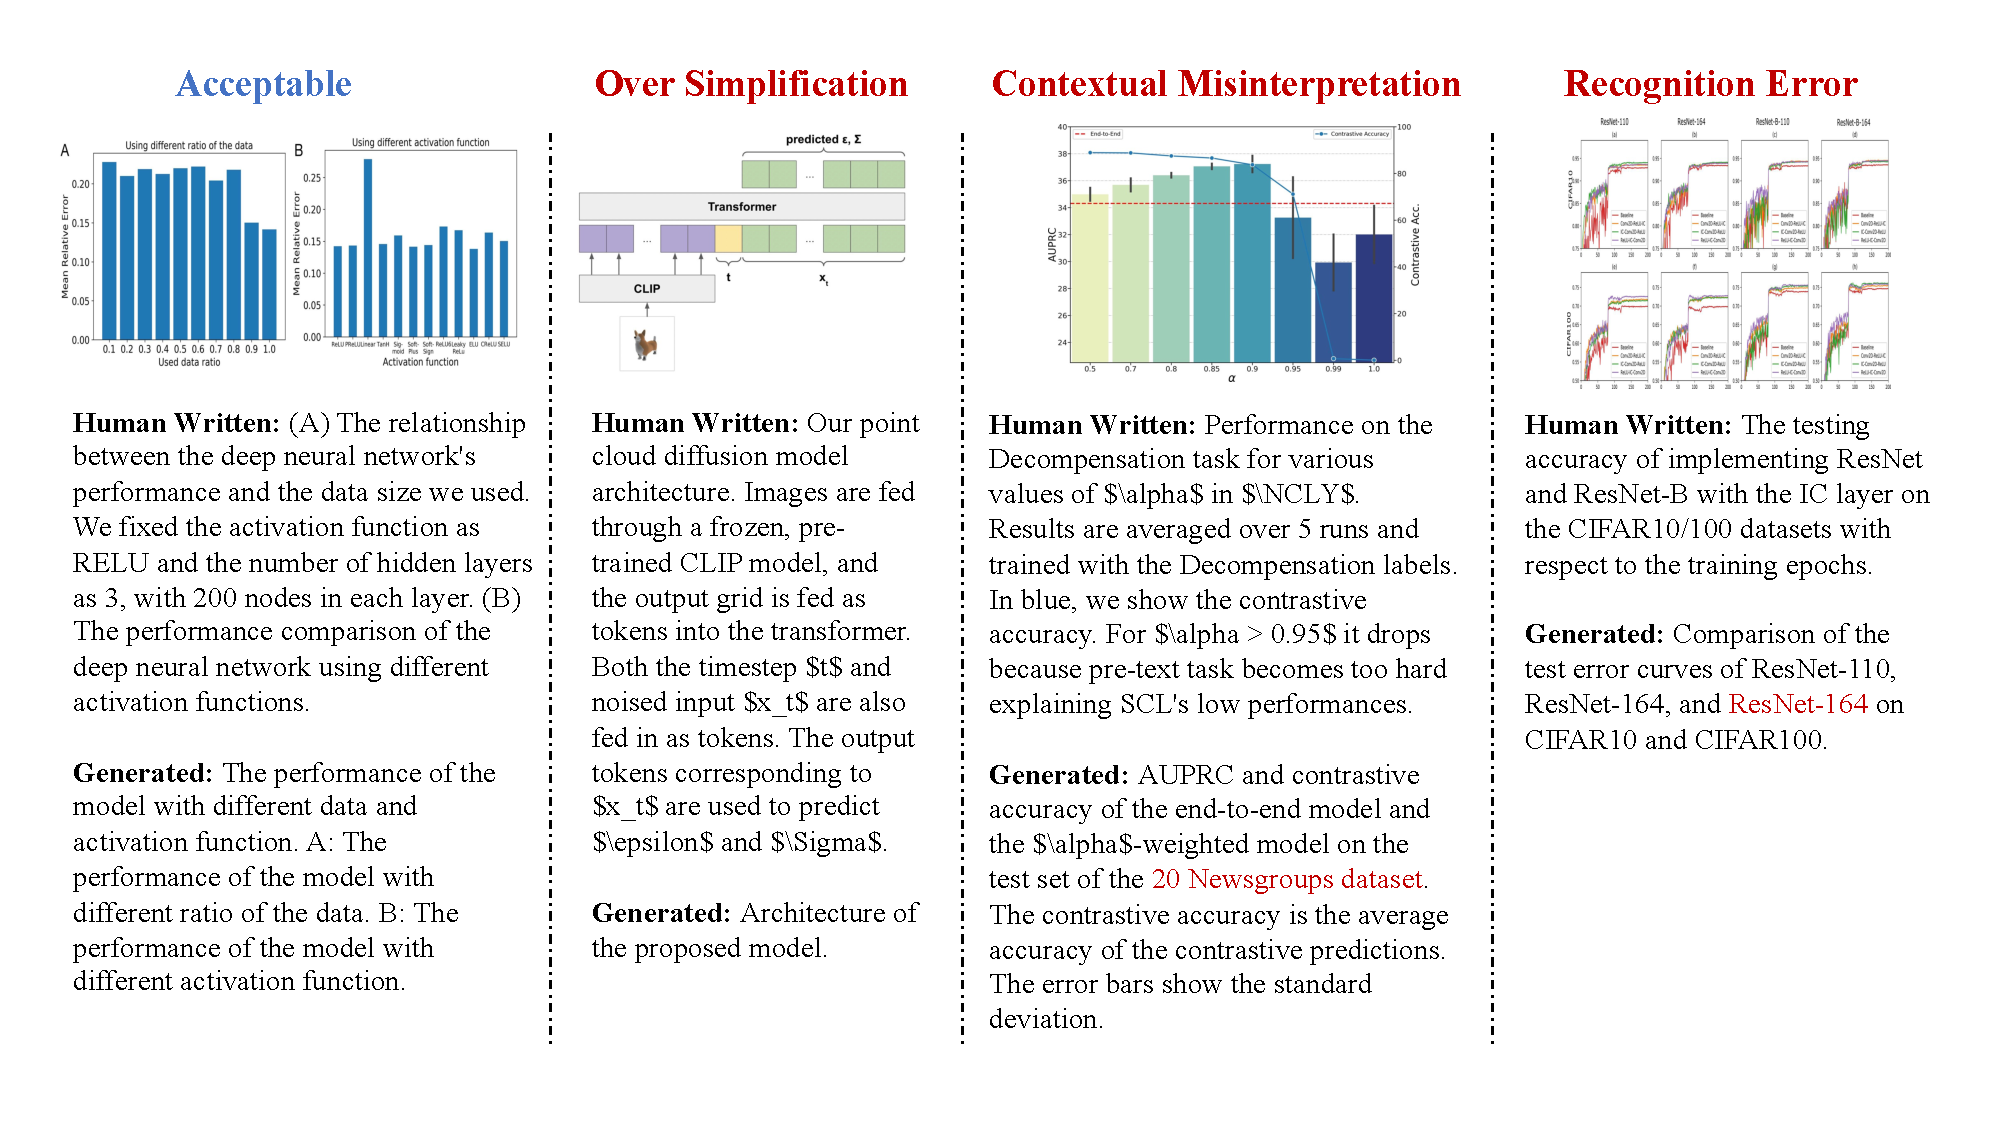
\includegraphics[width=0.95\linewidth]{figs/caption_error_type.pdf}
    \caption{Illustration of acceptable and three error types of generated captions.}
    \label{fig:caption_type}
\end{figure*}


\begin{figure}[t!]
    \centering
    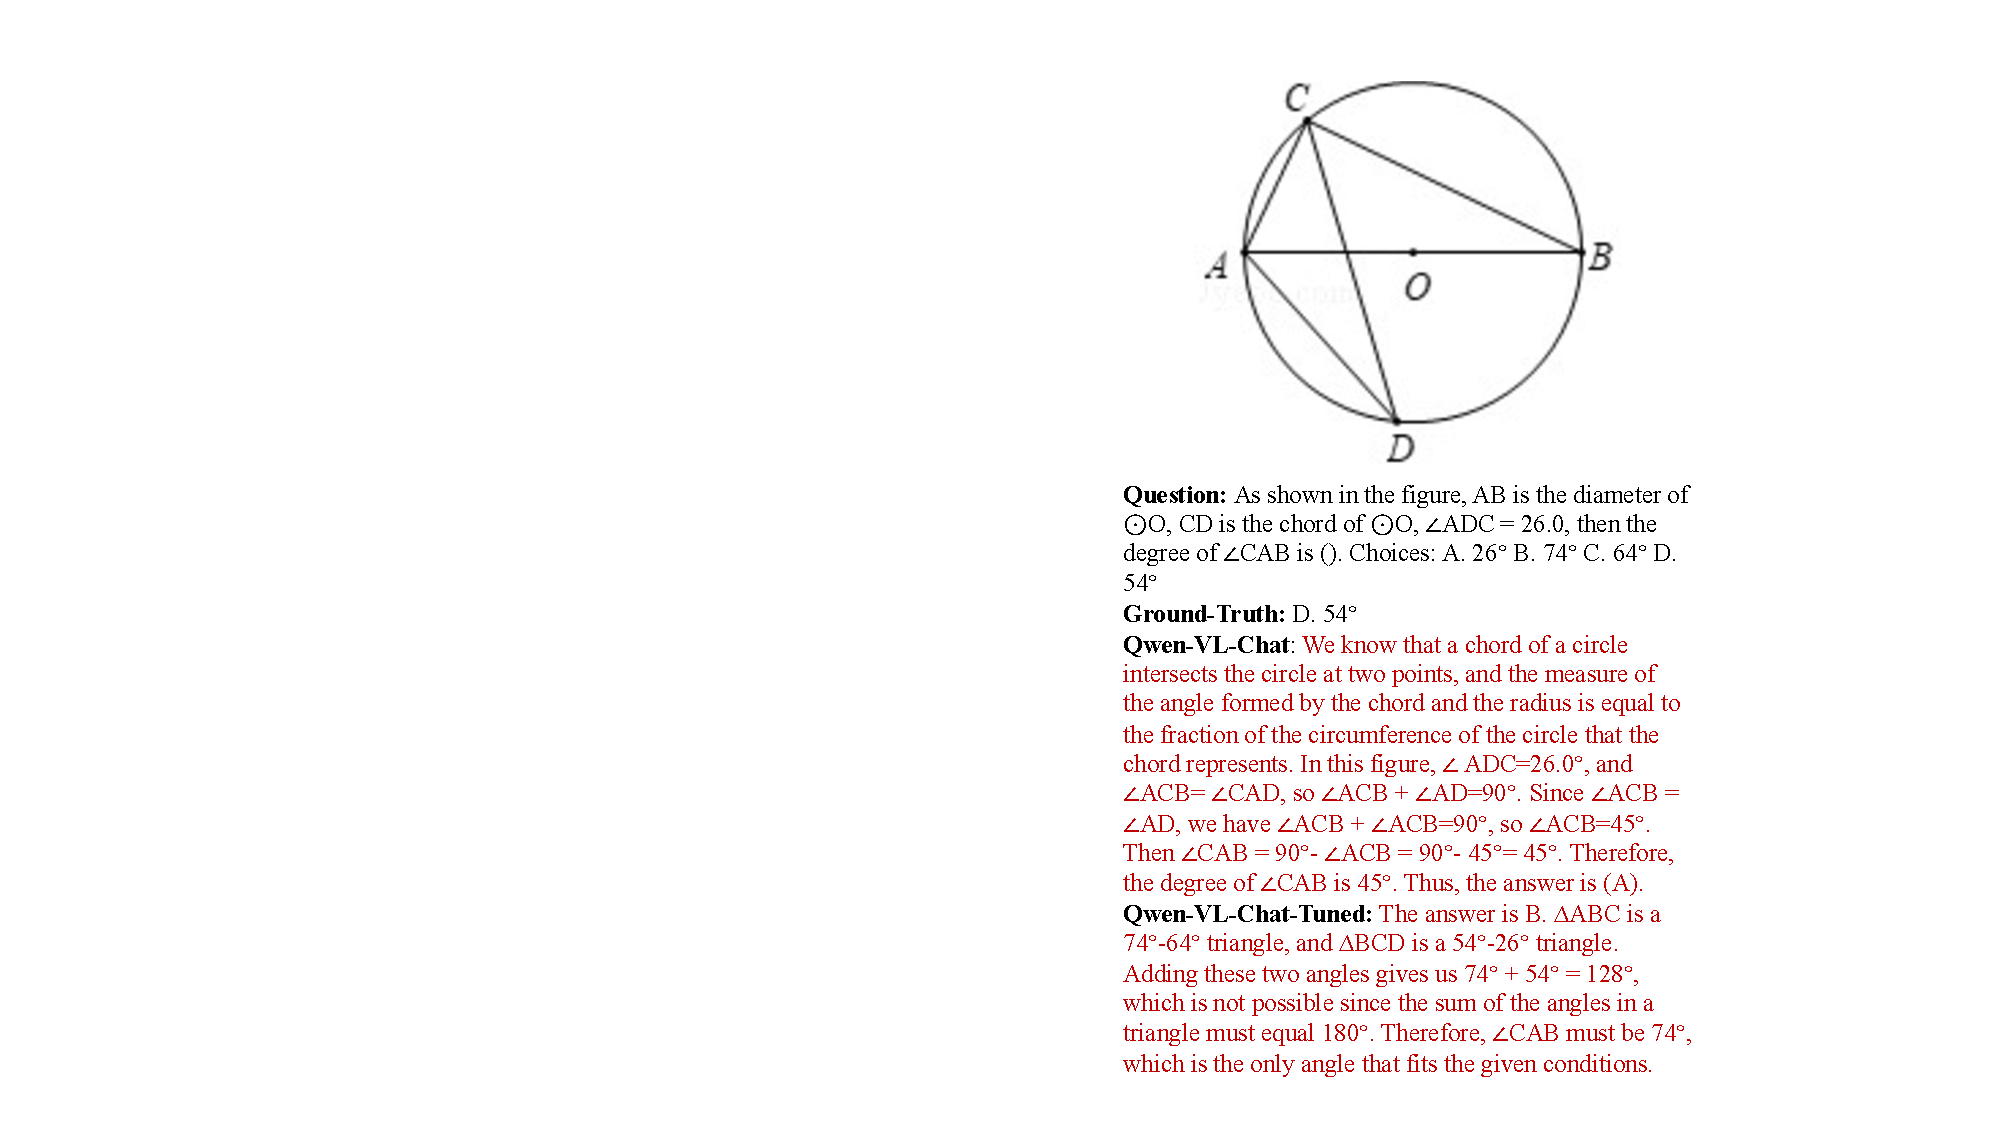
\includegraphics[width=0.85\linewidth]{figs/mathvista_both_wrong.pdf}
    \caption{A failure case on the geometry problem-solving task.}
\label{fig:geometry_fail}
\end{figure}
\subsection{Caption Type Illustration} 
\label{apx:caption_type}
We illustrate captions of four types in our main paper in Figure~\ref{fig:caption_type}. The \emph{Acceptable} caption provides a comprehensive description of the figure presented. The \emph{oversimplified} caption is too short compared with the original human-written caption. 
Furthermore, as shown in the third block in Figure~\ref{fig:caption_type}, \emph{Contextual Misinterpretation} refers to captions with unmentioned content in the figure, such as the dataset colored in red.
\emph{Recognition Error} denotes the model wrongly identified the number or text in the figure, such as the misidentified model name in the last block of Figure~\ref{fig:caption_type}.

\subsection{Failure Sample of MathVista}
\label{apx:failure_mathvista}
Figure~\ref{fig:geometry_fail} shows a challenging geometry mathematic reasoning problem where both models fail to produce the correct answer.
Echoing the quantitative results in our main paper, we believe future studies can incorporate more focused corpus for enhancing the geometry and mathematical reasoning ability of LVLMs.

\section{Results with LLaVA Backbone}
\label{apx:llava}

\begin{table*}[t!]
    \centering
    \small 
    \begin{tabular}{l|c c c c}
        \toprule
        Model & MathVista & MMMU(val) & ScienceQA(IMG only) & MM-Vet \\
        \midrule
        LLaVA-v1.5-7B & 26.6 & 35.3 & 66.8 & 30.5 \\
        \quad Original SFT +ArXivQA & \textbf{28.2} & \textbf{36.0} & \textbf{68.3} & \textbf{32.4} \\
        \bottomrule
    \end{tabular}
    \caption{After fine-tuning with a combination of ArXivQA and original SFT data, the LLaVA model shows boosted mathematical reasoning abilities across benchmarks.}
    \label{tab:llava_performance}
\end{table*}

We investigate whether ArXivQA could also enhance other LVLMs, such as LLaVA models~\citep{liu2023llava}. To maintain model performance, we mix our ArXivQA dataset with the LLaVA SFT 665K-instruction tuning dataset. The LLaVA-v1.5-7B is adopted as the backbone and the model is trained following the original recipe. The results on various benchmarks are listed in Table \ref{tab:llava_performance}.
We find that not only the scientific reasoning performance is improved on multimodal reasoning tasks (MathVista \citep{mathvista}, MMMU \citep{mmmu}, and ScienceQA \citep{lu2022scienceqa}), but the overall capability on MM-Vet \citep{yu2024mmvet} is also boosted. Together with our results using Qwen-VL-Chat, these findings indicate that our ArXivQA dataset can enhance different model backbones and is beneficial across various benchmarks.
\end{document}
